%\documentclass[final,subfig,blackref,approvalform]{drexel-thesis} %final copy
\documentclass[final,subfig,blackref,approvalform]{drexel-thesis} %final copy
%\documentclass[daring,subfig,blackref,draftspace]{drexel-thesis} %for committee
%\documentclass[daring,subfig,blackref,draftwatermark,draftspace]{drexel-thesis} %draft copy

%swap margins so the wide one is down the binding edge when printing double sided
%only use this with twoside
%\let\tmp\oddsidemargin
%\let\oddsidemargin\evensidemargin
%\let\evensidemargin\tmp
%\reversemarginpar

\usepackage{amsmath}
\usepackage{amssymb}
\usepackage{placeins}   % To allow pictures to flush after a section
\usepackage{setspace}
\usepackage{nth}
% \usepackage{tikz}
\usepackage{natbib}
\usepackage{multirow}
\usepackage{array}
\usepackage{soul}

\newcolumntype{C}[1]{>{\centering\let\newline\\\arraybackslash\hspace{0pt}}m{#1}}
\newcolumntype{L}[1]{>{\raggedright\let\newline\\\arraybackslash\hspace{0pt}}m{#1}}
\newcolumntype{R}[1]{>{\raggedleft\let\newline\\\arraybackslash\hspace{0pt}}m{#1}}

% fncychap clobbers \appendix with a silly implementation that breaks
% hyperlinks to appendix chapters.  Work around this by ignoring their
% implementation completely.
%\let\temporaryAppendix\appendix
%\usepackage[Conny]{fncychap}  % Nicer style used for distribution
%\usepackage[]{fncychap}
%\let\appendix\temporaryAppendix

%\usepackage[left]{showlabels}

\author{Jonathan F. Miller}
\title{TITLE}
\DUTmonth{MONTH}
\DUTyear{2015}
\degree{Doctor of Philosophy}
\advisor{Joshua Jacobs, Ph.D.}
% \includegra
% \copyrighttext{}


\renewcommand{\footrulewidth}{0pt}
\fancyfoot[RE,LO]{}
\fancyfoot[LE,RO]{}

\begin{document}

% !TEX root = ../thesis.tex
\begin{preamble}

\iffinal{}{\newpage}

\begin{DUTdedications}
\begin{center}
To Nicole.
\end{center}
\end{DUTdedications}

\iffinal{}{\newpage}

\begin{acknowledgments}
First and foremost, I'd like to thank and acknowledge my thesis advisor Joshua Jacobs. I've known Josh since I was an undergraduate and he was a graduate student at the University of Pennsylvania, over a decade ago. Through all of this time, even well before I knew I'd be his student, Josh has been a source of knowledge and guidance. Josh has taught me how to be a successful scientist, and, moreover, Josh has given me a set of skills that I am confident will serve me well in the future. I'm grateful to call Josh my friend, and I'm looking forward to our continued friendship over the years to come.

I am also indebted to Michael Kahana, who I've worked with for many years, and with whom I still collaborate. It was because of Mike that I first became interested in neuroscience, and it was through working in his lab as an undergraduate that I first began to understand the excitement that comes from trying to unravel the mysteries of the human brain. I would also like to thank many current and former members of the Kahana lab, in particular those who have helped me with the arduous task of data collection, including Emily Rosenberg, Erin Beck, Ryan Baily Williams, Patrick Crutchley, Ashwin Ramayya, John Burke, Deb Levy, and Anastasia Lyalenko. In addition, I'm grateful for my current lab members, notably Tom Coffey and Sang Ah Lee, for their invaluable support and insights over the course of my graduate career.

These acknowledgments would be incomplete without mentioning my clinical collaborators at Thomas Jefferson University Hospital, the Hospital of the University of Pennsylvania, UCLA Medical Center, and Freiburg University Hospital. It is through their efforts that I am afforded the rare opportunity to collect human neural recordings. I'd also like to thank the patients themselves from whom I've collected data, who selflessly volunteered to participate in our studies and who made this entire endeavor possible.

Lastly, I'd like to thank my wife Nicole Long, whose love and support has kept me focused, and my parents, for their unending encouragement.


\end{acknowledgments}

\iffinal{}{\newpage}

\tableofcontents 
\iffinal{}{\newpage}

\listoftables
\iffinal{}{\newpage}

\listoffigures 
\iffinal{}{\newpage}

\begin{abstract}
\ifdaring{\setstretch{1.3}}{\setstretch{1.6}}

The ability to navigate our environment is a vital skill for numerous species, including humans. How does the brain encode external space to allow for accurate navigation? Moreover, as we move through the world, how do we keep track of where specific events occur? Based on decades of research in rodents, we know that the hippocampus contains \textit{place cells} that code for particular locations in the environment, and based on decades of work in humans, we know that the hippocampus is crucial for episodic memory function. The goal of this dissertation is to study how the human brain simultaneously supports spatial navigation and memory function by analyzing intracranially recorded neural activity from participants performing virtual spatial memory tasks. In my first study, I investigated whether the neural representation of space formed by the place cell population code in the medial temporal lobe (MTL) becomes integrated with a broader memory signal. I found that place cells in human MTL act as a mechanism for memories to become linked to the location where they occurred, suggesting that the neural system underlying spatial navigation and the neural system underlying memory function are not as distinct as once thought.  In my next study, I investigated whether anatomical subregions of the human MTL, specifically the entorhinal cortex (EC) and the hippocampus, differ in the type of spatial information that they are selective to, which has been shown to be true in rodents. I discovered a new type of cell in the human EC called \textit{path equivalent cells} that provides a metric of distance relative to an environment's geometry, unlike hippocampal place cells that only fire at specific locations. This finding helps to bring our understanding of how space is represented in the human brain closer to our understanding of space in the rodent brain, which has been studied for many more decades. In my final study, I investigated how oscillatory activity in the human hippocampus is modulated by movement through the environment. In rodents, the \textit{theta} oscillation (4--10 Hz) is closely linked to voluntary movement through space and is an integral component for many rodent derived theories of MTL function. I found that functionally analogous signals in human hippocampus appeared at lower frequencies than in rodents, suggesting that these theories may require modification before they can be broadly applied to other species. Taken together, my work helps to reconcile how the MTL supports both spatial navigation and episodic memory function, as well as bridging the gap between the large literature describing the neural representation of space in the rodent brain and the comparatively less well understood mechanisms in the human brain.
\end{abstract}

\iffinal{}{\newpage}

\end{preamble}




























\begin{thesis}
  % \pdfbookmark[-1]{Main Matter}{Main Matter}
  % \ifdaring{\setstretch{1.3}}{}
  %\ifdaring{\setstretch{1.3}}{\setstretch{1.3}}
  
    % CHAPTER 1: Introduction
    % !TEX root = ../thesis.tex
\chapter{Introduction}
% \large

As we move through our lives, we also move through the world. We go from room to room within our homes, we commute from our homes to our workplace, we travel throughout our neighborhoods and cities, and we take vacations to explore new countries. As we move, we learn our way around our environment. We create an internal map - an internal representation of external space - that allows us to get from place to place, and, in addition, provides us with the means to keep track of where the events that we experience in our lives occur. We have the ability to both navigate our world and to form rich detailed memories as we move through it. Somehow, our brains support these dual abilities, which are fundamental to our daily quality of life.

Decades of neuroscience research have attempted to uncover the neural mechanisms responsible for spatial navigation and memory function, yet these two fields have largely been studied independently from each other. The investigation into the neural basis of spatial navigation was propelled forward over 40 years ago by the discovery of \textit{place cells} in ambulating rats \citep{OKeeDost71}. Place cells are neurons, primarily located in the hippocampus, that fire action potentials whenever the animal is physically located at a particular spot in world. They are remarkable in that they reveal a clear mapping of external space onto a neural substrate, and they provided the first indication as to how the brain might create an internal, or cognitive, map of our surroundings. This finding, which has since earned discoverer John O'Keefe the 2014 Nobel prize in Physiology or Medicine, spawned an entire subfield of neuroscience focused on detailing the neural representation of space in the rodent hippocampus and the surrounding medial temporal lobe structures of the brain.

In contrast, our understanding of the neural underpinnings of memory function is rooted in human neurophysiology. When patient H.M.\ had his hippocampi removed to treat his medication-resistant epilepsy, he could no longer reliably form new memories \citep{ScovMiln57}. More specifically, he could no longer form new \textit{episodic} memories, or memories for experienced events \citep{Tulv72}. As with rodents and place cells, this discovery of a clear functional relationship between a neural structure -- once again, the hippocampus -- and an observable behavior served to focus much of the field's future attention. In this case, it was focused on the role of the human hippocampus in supporting episodic memory function.

The fact that the same neural structures underly both spatial navigation and declarative memory abilities caused two schools of thought to emerge, one that believes that the hippocampus is primarily spatial in nature \citep{OKeeNade78,HartEtal14}, and another that believes the hippocampus' core role is to support mnemonic processing \citep{CoheSqui80}. In spite of this historical delineation, the spaces we inhabit and the memories we form within those spaces are intricately linked. When we reimagine the past, be it what we had for breakfast today or a favorite childhood birthday party from decades prior, the location of the past event is one of the primary and salient features of the memory.  Recent work, recognizing this link between space and memory, has attempted to reconcile the opposing views by suggesting that that the hippocampus isn't specific for memory or space per se, but rather comprises a flexible ``memory space'' that adapts to current spatial or non-spatial demands \citep{EichEtal99,EichCohe14}. A main goal of the research described in this dissertation is to further bridge the divide between these areas of research, spatial navigation in rodents and memory for past events in humans, and simultaneously study spatial navigation and memory function using human neural recordings. In order to do so, I will first describe certain methodological details upon which my work is based, including how the neural data is collected and how human navigation and memory can be probed in an experimental setting.

% Despite the
% As will be discussed, the reasons for this delineation are both historical and the result methodological limitations that have only recently been overcome. A primary goal of the work described in this dissertation is to bridge this divide and simultaneously study spatial navigation and memory function using human neural recordings.

% The neuroscience of memory 



% focus on hippocampus/mtl
% ieeg / microelectrodes
% episodic memory
% spatial navigation
% theta
% vr


% When we reimagine the past, be it what we had for breakfast today or a favorite childhood birthday party from decades prior, the location of the past event is one of the primary and salient features of the memory. 


\section{Human intracranial recordings}

Rodent place cells were discovered by recording \textit{in vivo} activity from individual neurons using electrodes inserted into rodent hippocampus. To facilitate making comparisons to rodent research, the studies I perform here all make use of the rare opportunity to collect intracranial recordings of neural activity from electrodes implanted directly in the human brain. For clear ethical reasons, recording neural activity from the general population using direct brain implants is not justifiable. As a result, this work relies on data from the population of epilepsy patients who are undergoing monitoring for seizure localization. These patients all suffer from seizures that cannot be controlled though pharmacological intervention, thus they have elected to have electrodes placed subdurally (on the surface of the cortex) as well as to have electrode depth probes inserted into deeper brain structures, such as the hippocampus.

The goal of this procedure is to localize the area of the brain responsible for the generation of seizures, with the aim of ultimately resecting the seizure focus to reduce or eliminate seizure production. Patients remain in the hospital for $\sim$1--3 weeks while their brain activity is being recorded. The data collected using this method, known as either intracranial electroencephalogic (iEEG) or electrocorticographic (ECoG) recordings, provide the clinicians with a means of assessing which areas of the brain are epileptogenic, and the procedure results in significant reduction in seizure frequency in approximately 50\% of patients \citep{WiebEtal01}. 

When patients are not occupied with clinical matters, they are often free to participate in cognitive studies, affording researchers a unique opportunity to measure the electrical activity of the brain recorded via direct contact with active tissue. The data collected with this methodology can be broken down into two distinct categories. First, one can analyze the signals recorded from macroelectrodes, which are relatively large contacts with diameters measured in the range of millimeters. These contacts record the activity of a $\sim$4mm$^{2}$ area of tissue, encompassing the summed activity of a large population of neurons. Signals recorded from these macroelectrodes are generally analyzed by either examining how the voltage potential changes as a function of experiment condition, or by decomposing the voltage time series into its constituent frequencies and determining how the power and phase of the signal at various frequencies is related to experimental conditions of interest.

The second type of data is collected from microelectrodes, which are much smaller than macroelectrodes, having diameters in the range of microns (in the case of the studies performed here, the microelectrodes have a diameter of 40$\mu$m). Microelectrodes extend from the tip of the depth probes inserted into deep brain structures, and, importantly, are small enough to measure the action potentials of individual neurons. Here, the unit of analysis is not necessarily the voltage or power signal, but is rather the timing and rate of neuronal spiking. This spiking data is analogous to the type of data that led to the discovery of place cells in rodents, allowing for similar analytic methods to be carried out with human data. 

% \hl{MAKE FIGURE WITH VOLATE TRACE HERE? or not necessary?}

% As a result, non-invasive techniques to study the relationship between brain activation and cognition such as functional magnetic resonance imaging (fMRI) dominate the field of cognitive neuroscience. However, while fMRI has proved to be an invaluable, and due to to its accessibility, very popular,  neuroscience tool, its utility is limited 

\section{The neural representation of space}

% The work described in this dissertations, in particular in Chapters 2 and 3,

When place cells were discovered and their properties first studied in the 1970s, researchers had their first glimpse into the precise neural mechanisms supporting an organism's ability to self-localize within the external environment. Place cells, with their well-defined ``place fields'' that link a physical location to an internal representation \citep{OKeeNade78}, suggested a  concrete mechanism by which the brain stores a map of the world. With a large enough set of place cells, each one coding for a particular region of space, an animal's location at any given moment can be represented by the activity of the population of cells. Indeed, if enough simultaneous place cells are recorded, a rodent's position can be accurately reconstructed from the neural activity \citep{WilsMcNa93,ZhanEtal98}. For a time, it seemed as though a pure cognitive map, as hypothesized by Edward Tolman decades prior \citep{Tolm48}, had been found.

Over time, however, it has become clear the spatial representation system in the brain is much more complex. Not only are there place cells in the hippocampus that code for particular locations, but there are numerous other types of cells throughout the medial temporal lobe (MTL) that are tuned to specific environmental properties. For example, head direction cells in pre- and parasubiculum code for the direction the animal is facing \citep{TaubEtal90}, border or boundary cells in the entorhinal cortex (EC) code for locations near the edge of an environment \citep{SolsEtal08}, and grid cells in the EC have non-localized firing fields that tessellate across an entire region of space \citep{HaftEtal05}.

In addition to these specialized cell types, brain oscillations -- the result of the summed activity of populations of neurons \citep{LachEtal03} -- are closely tied to rodent spatial navigation. Of particular interest is the hippocampal \textit{theta} oscillation, typically defined as 4--10 Hz, whose amplitude increases during periods of voluntary movement \citep{Vand69}. Moreover, theta is mechanistically related to the activity of spatially tuned cells. The theta oscillation is thought to play a key role in coordinating the timing of action potentials of place cells, such that the likelihood of firing varies as function of the phase of theta \citep{OKeeRecc93,SkagEtal96}. Oscillatory interference models of EC grid cell generation causally rely on theta when explaining how grid cells are formed \citep{BurgEtal07}, and, moreover, rodent work has shown that chemically induced inactivation of the theta signal disrupts grid cell firing patterns \citep{KoenEtal11,BranEtal11}. The diversity of spatially tuned cells and their modulation by oscillatory activity raises questions about how all of this information is integrated and what roles different MTL structures may play in supporting navigation abilities.

In contrast to the large volume of work describing the neural representation of space in the rodent brain, there has been relatively little work investigating the same questions in humans. Place cells and grid cells have indeed been shown to exist in human MTL \citep{EkstEtal03,JacoEtal10,JacoEtal13}, and low frequency oscillations are more prominent during periods of movement \citep{CaplEtal03,KahaEtal99}. However, our knowledge of how the human brain represents external space still pales in comparison to our knowledge of rodents. Do the properties of spatially tuned cells vary based on brain region? Does the theta oscillation, with its strong functional ties to navigation in the rodent, act in an analogous manner in humans? Furthermore, with so much of the MTL seemingly dedicated to spatial processing, reconciling how the same part of the brain is vital for memory function in humans has been a challenge. An aim of my work is to investigate these issues in humans with a level of detail approaching that done in rodents.


% with so much spatial specific stuff, what about memory?

% also theta

% also some human stuff, we will build off it

\section{Episodic memory and spatiotemporal context}

Space is an intuitively vital aspect of our episodic memories. The events that we experience in our lives necessarily occur at a particular time, with particular surroundings, and at a particular location. This can be framed more formally by saying that events take place within a \textit{spatiotemporal} context, such that we can remember both where and when an event occurred \citep{Tulv83,Eich04}. Yet, throughout the history of episodic memory experiments, the study of the role played by spatial information has largely been ignored. In general, episodic memory experiments present study participants with lists of words or pictures to encode so that they can later be recalled or recognized, devoid of any spatial information. Thus, a major drawback of these traditional methods is that they lack a sense of real world ecological validity, as it has been shown that spatial information is a key element in memory formation, organization, and retrieval \citep{MillEtal12a}. To overcome this limitation of previous studies, all of the work I will present makes use of virtual environments to extend experiments into three dimensions, allowing for the study of the neural representation of space, memory, and their interactions.

\paragraph{Virtual navigation} 

To study the neural representation of space in the rodent, researchers generally record from a freely moving animal that is tethered to a recording system. Unfortunately for human research, the ability to record from the human brain comes with the cost of limited mobility. When hospital patients perform iEEG experiments, they are either resting in their bed or sitting in their chair. To overcome this restriction, we create visually rich 3D environments that participants navigate on a laptop computer. While virtual tasks lack the locomotive and proprioceptive feedback of real navigation and do elicit somewhat diminished spatial selectivity \citep{ChenEtal13,RavaEtal13}, previous studies of both rodent \citep{HarvEtal09,ChenEtal13} and human \citep{EkstEtal03,JacoEtal10,JacoEtal13} spatial navigation have revealed that virtual navigation is sufficient to elicit neural responses that generally similar to actual navigation in rodents. In addition, though we lose certain attributes of real world navigation, we gain the capability to precisely design and control the virtual environments to our exact specifications.

The virtual environments that I will describe were created using the Panda Experiment Programming Library (PandaEPL), which is an open source 3D experiment platform \citep{SolwEtal13}. PandaEPL allows for the construction of freely navigable 3D environments, and importantly, incorporates extremely precise logging to accurately align patient activity in the task with the neural data.

% Much of the work discussed in this dissertation attempts to help us understand how the human brain supports episodic memory, with a focus on the spatial component of memory episodes.

% place cells can thought of in a memory orientated way

% \section{From rodents to humans}

% or is that here?

\section{Overview}

% episodic memory important, can only really be tested in humans
We are all defined by our memories and past experiences, of which space is a core component. This is perhaps most evident when considering the profound effects of neurodegenerative diseases such as Alzheimer's, where the loss of memory function, along with spatial disorientation, are primary symptoms. As we move through space and time, we are constantly encoding new memories for later retrieval, transforming the events of our lives into patterns of brain activity. Understanding the neural underpinnings of this process is a lofty yet fundamental goal of neuroscience.
% and it is a goal that can only truly be accomplished through the study of the human brain. Whether or not any animals possess episodic memory in a manner that is on par with humans is an open debate \citep{ClayEtal03}, yet is is hard to dispute the fact that only humans possess the combination of episodic memory, language, and communication abilities necessary for performing in-depth experiments of memory function.
Whether or not any animals possess episodic memory in a manner that is on par with humans is an open debate \citep{ClayEtal03}, yet is is hard to dispute the claim that this goal, due to our combination of memory, language, and communication abilities, can only truly be accomplished through the study of the human brain.

The body of work that I will present is focused on two overarching themes. First, my work serves to extend our knowledge of how the brain represents spatial information by studying spatial navigation in humans. Directly comparing rodent findings with data from human studies is necessary in order to validate theories of brain function that are derived mainly from the rodent literature. Second, I make use of the fact that memory in humans can be probed more explicitly than memory in animals to investigate how the brain represents the spatial components of memories, as well as to better understand what role these components may play in the general episodic memory engine.

In \textbf{Chapter 2}, I build upon our knowledge of the existence of place cells in humans to examine if place cells are simply an internal biomarker of location or whether they become integrated into a broader memory trace. To do so, I recorded the activity of individual medial temporal lobe neurons in patients performing a hybrid memory and spatial navigation task, and I found that place cells that were active during spatial navigation reactivated outside of navigation when patients recalled specific memory episodes. In \textbf{Chapter 3}, I add to our understanding of how the brain represents space through the discovery of new type of spatially tuned cell not previously seen humans. I show that \textit{path equivalent cells} encode distance traveled relative to environmental geometry, and, in line with rodent findings \citep{FranEtal00}, that these cells tend to be localized to the entorhinal cortex. In \textbf{Chapter 4}, I use analyses of oscillatory activity to investigate whether the key role played by theta oscillations in rodent navigation and memory is conserved across species. While I found that many core attributes translated from rodents to humans, there do exist fundamental inter-species differences in the behavior of movement related oscillatory activity, highlighting the need to validate existing theories using human data. In \textbf{Chapter 5}, I synthesize these findings and relate them to the broader literature of both spatial navigation and memory function.

% In chapter 3, I extend our knowledge of the human neural representation of space, which further links rodent and human literature and gives us insight into the precise roles of MTL regions. New cell type is a key advancement of the field.
% 
% In chapter 4, I more precisely compare core findings from rodent navigation with human data from a optimized task. some similarities, but some differences with important theoretical implications.

% - Chapter 2: spatial components of episodic memories. context reinstatement.
% - Chapter 3: ec repeating spatial activations. non-specific vs hipp specific.
% - Chapter 4: role of theta in movement compared to rodents. Also memory..


    % CHAPTER 2: Miller et al., 2013
    \chapter{Neural Activity in Human Hippocampal Formation Reveals the Spatial Context of Retrieved Memories}
    \begin{quotation}
    \singlespacing
    \noindent Jonathan F. Miller, Markus Neufang, Alec Solway, Armin Brandt, Michael Trippel, Irina Mader, Stefan Hefft, Max Merkow, Sean M.  Polyn, Joshua Jacobs, Michael J. Kahan, \& Andreas Schulze-Bonhage  \\ \textit{Science}
    \end{quotation}
    
\section{Abstract}

In many species, spatial navigation is supported by a network of ``place cells'' that exhibit increased firing whenever an animal is in a certain region of an environment. Does this neural representation of location form part of the spatiotemporal context into which episodic memories are encoded? We recorded medial temporal lobe neuronal activity as neurosurgical patients performed a hybrid spatial and episodic memory task.  We identified place-responsive cells active during virtual navigation and then asked whether the same cells activated during the subsequent recall of navigation-related memories without actual navigation. Place-responsive cell activity was reinstated during episodic memory retrieval. Neuronal firing during the retrieval of each memory was  similar to the activity that represented the locations in the environment  where the memory was initially encoded.


\section{Introduction, Results, and Discussion}
When one encounters an old friend and remembers the time they last met, often the place of meeting and surrounding circumstances come to mind. This is the hallmark of episodic memory---the capacity to store and later retrieve memories that are bound to a particular place and time \cite{Tulv83}.  Theories of episodic memory posit that the brain supports this ability by continually maintaining an updated representation of the current spatiotemporal context, which is a neural representation of space, time, and other aspects of one's current cognitive milieu \cite{PolyKaha08}.  When the brain forms a new episodic memory, these theories predict that the content of the experience becomes associated with the current spatial and temporal context.  When the memory is retrieved, this prior context is partially reinstated, focusing one's thoughts on time and place of the remembered episode. This reinstatement not only provides the phenomenological experience of remembering, but it also helps to cue other memories experienced within the same or related contexts.

Although it is well established that the hippocampus and surrounding medial-temporal-lobe (MTL) structures play a central role in the formation and retrieval of context-mediated memories \cite{ScovMiln57,Eich04,Dava06}, we know far less about how these memory processes manifest in the activities of individual MTL neurons.  Much of what is known about the neural coding properties of hippocampal and MTL neurons comes from studies of rodent spatial navigation, where individual neurons respond preferentially at specific  locations within a given contextually-defined spatial environment  \cite{OKeeNade78,McNaEtal06}.  Similar neuronal responses have also been identified in the human hippocampus during virtual spatial navigation \cite{EkstEtal03,JacoEtal10}.  The context dependent firing of these neurons \cite{MullKubi87,LeutEtal05} and their dependence on the animal's goal state or past history of experienced cues \cite{WoodEtal00,FerbShap03} has led some to speculate that the neural representation of space in the hippocampus is  part of a broader network of neurons that encode episodic memories more generally \cite{EichEtal99,Buzs05,HowaEtal05,BuzsMose13}.  This hypothesis suggests that the same neural structures and computations that enable the learning of a spatial layout via place cell activity also facilitate encoding episodic memories. However, according to a prominent alternative account, the spatial coding functions of the hippocampus are part of a context module that operates independently of the computations that encode the content of a memory \cite{DavaEtal03,HargEtal05}.

\begin{figure}
  \begin{center} \centering
    \includegraphics[width=.8\textwidth]{./tex/dboy/figs/fig1}
  \caption[\emph{Delivery Person} task design]{The behavioral task. \textbf{A.} Overhead map of the virtual environment. Red rectangles indicate store locations, and blue squares indicate locations of non-store buildings. Green areas indicate grass and trees, and the small dark blue, brown, and yellow boxes represent mailboxes, benches, and street lights. \textbf{B.} An example storefront that a subject might encounter. \textbf{C.} The presentation of an item (a zucchini) upon arrival at the target store (bakery). \textbf{D.} The initiation of the recall period, as indicated by a black screen with asterisks.}
\label{fig:dboy_town}
\end{center}
\end{figure}

We designed a virtual-reality memory game in which subjects played the role of a delivery person, driving through a virtual town and delivering objects to stores.  Our subjects were patients with drug resistant epilepsy who were implanted with depth electrodes to localize the focus of their seizures and to map cognitive function in surrounding healthy tissue. In an initial phase of the game, subjects explored the town using a computer controller to navigate from store to store as they attempted to learn the layout of the environment illustrated in Fig.~1A.  After this initial familiarization phase, during which subjects visited each store twice, they began a series of ``delivery days''.  On each delivery day, subjects were instructed to travel from store to store, visiting 13 randomly chosen stores (of the 16 total) in a randomly determined order.  Upon their arrival at each store, they were presented with an object (either visually for 2 sec for subjects 1 - 5 or aurally for subjects 6 - 7).  Upon arrival at the final (13th) store, no item was presented. Instead, the screen went black and subjects were prompted to vocally recall as many of the 12 delivered objects as they could remember in any order (subjects recalled 5.2 objects, on average).  After being given 90 seconds for free recall, subjects could advance to a new delivery day, in which they would deliver a unique but randomly determined set of objects to a random sequence of 13 stores and then attempt to recall the new set of objects. Consistent with prior work \cite{MillEtal12a}, subjects exhibited a significant ($p=.008$) tendency to consecutively recall objects delivered to more spatially proximate locations (see supplementary online materials (SOM) text).

% \section{Results}
% 
We first sought to identify patterns of neuronal activity that represented subjects' location within the virtual town. We identified place-responsive cells as the neurons that exhibited significantly increased firing at a particular location in the virtual environment. Fig.~2A depicts the activity of one example place-responsive cell, which increased its firing rate when the subject was positioned at a location on the left side of the virtual environment and facing north.  The majority of the identified place-responsive cells were direction dependent (72\%) and did not exhibit significant place fields when direction of traversal was not taken into account.  This is similar to prior findings of directionally oriented place cells in environments with clearly defined routes, in contrast to open environments, where omnidirectional place cells are prevalent \cite{MullEtal94,EkstEtal03}.  These directionally-oriented place cells were not generally responsive to place-invariant view information. Fig.~2B shows the firing rate of a place-responsive cell from the entorhinal cortex, which activated at a location in the south part of the environment during eastward movements.  In total, we identified 95 place-responsive cells, comprising 25.6\% of all observed neurons. There were significant numbers of place-responsive cells in the hippocampus, entorhinal cortex, amygdala, and in anterior MTL regions of ambiguous localization (binomial test with $p<0.01$ for each region, Fig.~2C, Tables S1 and S2).

\begin{figure}
\centering
    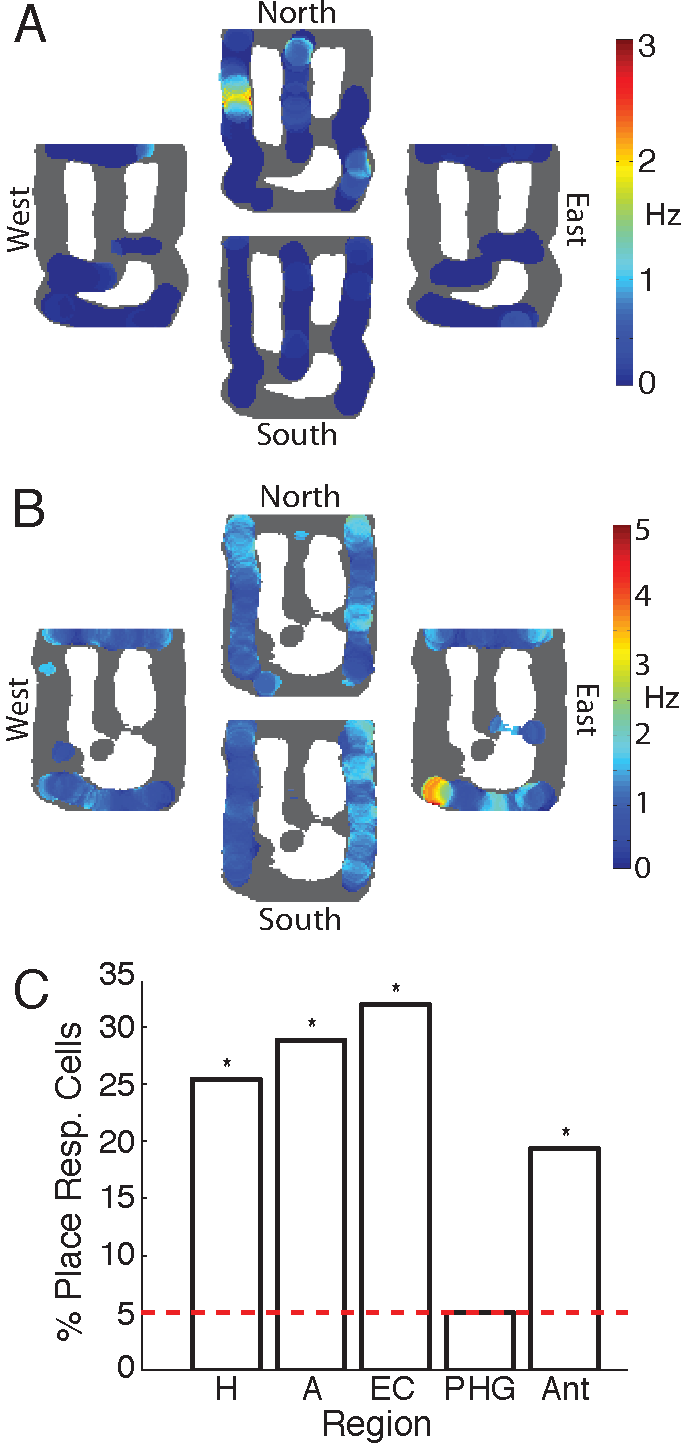
\includegraphics[width=.5\textwidth]{./tex/dboy/figs/fig2}
  \caption[Place-responsive cells]{Place-responsive cells.  \textbf{A}. Firing rate map for a cell responsive to northward traversals located in Subject 6's hippocampus, shown separately for each cardinal direction. Grey represents all areas traversed by the subject, regardless of direction of travel. \textbf{B.} A cell responsive to eastward traversals recorded from Subject 1's entorhinal cortex. \textbf{C.} The regional distribution of place-responsive cells in the entire dataset of 371 single units (H: hippocampus, A: amygdala, EC: entorhinal cortex, PHG: parahippocampal gyrus, Ant: anterior MTL, not otherwise specified).  The red line indicates the false positive rate of 5\%.}
\label{fig:place_ex}
\end{figure}

To determine whether spontaneous retrieval of items during free recall reinstated the spatial context associated with the item's encoding, we calculated the neural similarity between ensemble place-responsive cell activity during navigation and during item retrieval (see Fig. S1 for further details).  We partitioned the environment into three regions for each recalled item: regions close to the delivery location, regions of intermediate distance, and regions that were far from the delivery location.  We then asked whether the ensemble place-cell activity at the time of retrieval was more similar to navigational epochs that were closer to the delivery location.  A high degree of similarity would indicate the reinstatement of the spatial context associated with the item.  To protect against potential confounding between object and spatial context, we excluded navigational epochs surrounding the delivery of an object.  

We found significant spatial context reinstatement surrounding the time of item vocalization (timecourse illustrated in Fig.~3A). The level of neural similarity between recall activity and navigation activity was ordered such that areas of the environment near  an item's encoding location exhibited the highest similarity scores, intermediate spatial distances exhibited middling similarity scores, and far spatial distances exhibited the lowest similarity scores (this effect being strongest in the -300 to 700 ms interval illustrated in Fig.~3B).  An ANOVA indicated a significant effect of distance bin on the level of neural similarity ($F$(2,300) = 7.6, $p <$ .001). Performing this latter analysis across subjects rather than recall events revealed that neural similarity within the near distance bin was significantly greater than neural similarity within the far distance bin (Fig.~3C, $t$(5) = 4.0, $p =$ .009).   

\begin{figure}
\centering
  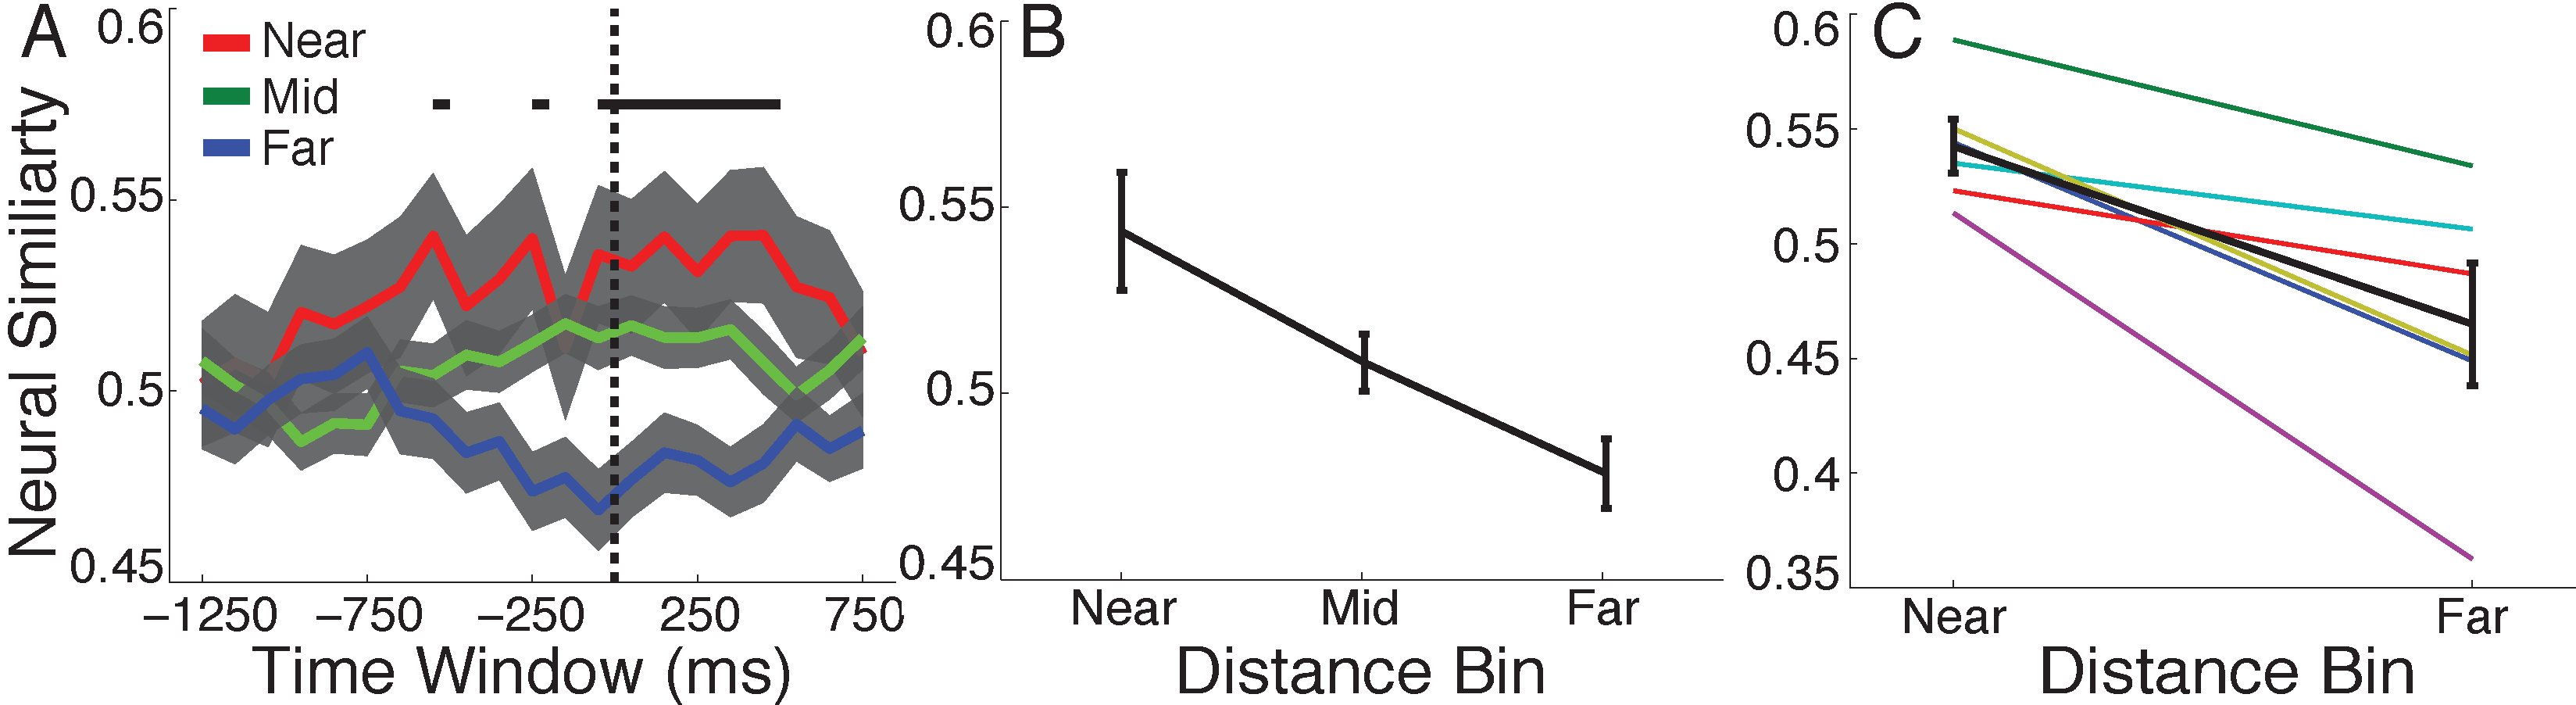
\includegraphics[width=1\textwidth]{./tex/dboy/figs/fig3}
  \caption[Timecourse of neural similarity]{\textbf{A.} Timecourses of neural similarity between ensemble place cell activity during navigation and during item recall are shown for near, middle, and far spatial distance bins.  Timecourses, shown relative to recall onset, were  computed in overlapping 500-ms windows (x-values indicate the center of the window).  Similarity is defined as the cosine of the angle between ensemble activity during recall and navigation, normalized as a rank score. Shaded regions indicate standard error of the mean across recalled items. The horizontal bar indicates significant timepoints as determined by an ANOVA with a false discovery rate adjusted significance threshold of 0.017.  \textbf{B.} The average neural similarity for near, middle, and far spatial distance bins are shown for the time period -300--700 ms relative to recall onset. Error bars indicate standard error of the mean across recalled items.  \textbf{C.} The neural similarity for near and far spatial distance bins for each of the included subjects (thin colored lines) and the subject average (thick black line) are shown for the  time period -300--700 ms relative to recall onset. Error bars indicate standard error of the mean across subjects.}
\label{fig:reinstate}
\end{figure}

During the spontaneous recall of an item, place-responsive cells exhibited firing patterns similar to those they showed during exploration of the region of the town where the item was previously delivered.  Thus, recalling an episodic memory involves recovery of its spatial context, as seen in the activity of place-responsive cells in the human hippocampal formation and surrounding MTL regions. If the object delivery occurred in or near a cell's place field, characterized by a significantly higher than baseline firing rate, then recalling the object should also produce an increase in firing rate. We calculated the firing rate of place-responsive cells when subjects were navigating inside and outside of each cell's place field, as well as the firing rate when subjects recalled items that were presented near to or far from each cell's respective place field (Fig.~4) (see Fig. S2 for further details).  The average in-field firing rate (3.8 Hz) was substantially higher than the out-of-field firing rate  (1.9 Hz; $t$(32) = 5.9, $p < 10^{-5}$).  The average firing rate during the recall of items presented near a place field was 2.2 Hz, which was significantly higher than the 1.8 Hz firing rate during recall of items presented far from a place field ($t$(32) = 2.2, $p =$ .03).

% \section{Discussion?}

Unlike traditional list recall studies of episodic memory, where items unfold only in time, the present experiment provided a unique spatial context for each item.  This allowed us to leverage the  spatial-coding properties of hippocampal neurons in the study of the neural basis of episodic recollection.  Spatially-sensitive neural activity in the hippocampal formation became reactivated during episodic retrieval, when no visual cues were present.  At the time of recall, subjects simply vocalized the names of the delivered objects in the order they came to mind, yet the neurons responsive to spatial  information reactivated during the time just before and during vocalization.  This reactivation implies  that  each experienced item is bound to its spatial context, which in turn may be reinstated when the item comes to mind during recall.  

\begin{figure}
\centering
  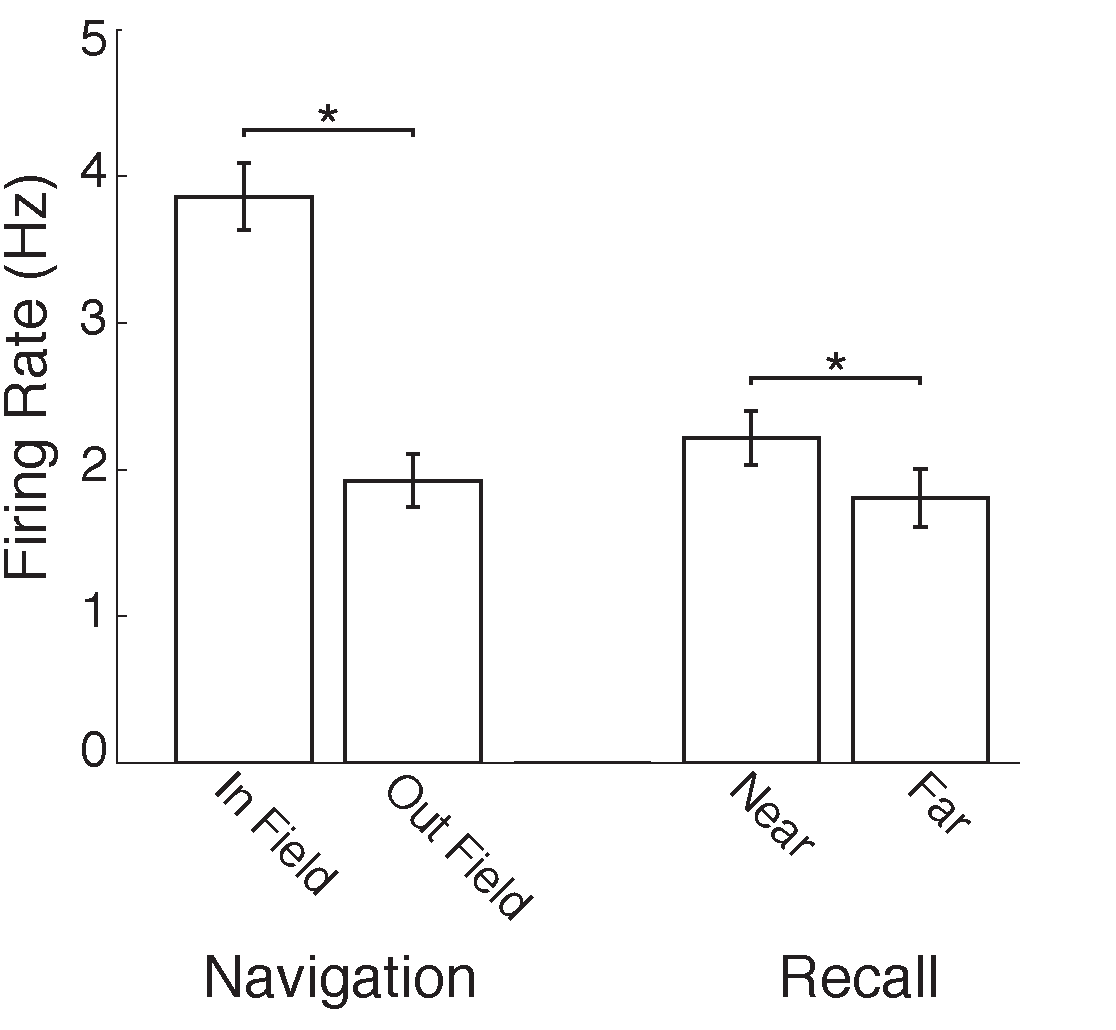
\includegraphics[width=.6\textwidth]{./tex/dboy/figs/fig4}
  \caption[Place-responsive cell firing rate by condition]{Place-responsive cell firing rate by condition. \textbf{Navigation.} In Field indicates the average place-responsive cell firing rate when navigating within a cell's place field, whereas Out Field indicates the average place-responsive cell firing rate at locations outside of a place field ($p < 10^{-5}$). \textbf{Recall.} Near indicates the average place-responsive cell firing rate in time period -1.5 s before to 1 s after recall onset of items that were initially presented in or close to the center of a place field, and, in contrast, Far represents the average place-responsive cell firing rate in the same time window for recall of items that were initially presented far from the center of a place field ($p =$ .03).}
\label{fig:fr_by_cond}
\end{figure}

Because human neural recordings are rarely possible, little is known about the neural substrates of spontaneous verbal recall.  Nonetheless, several recent studies have established the general phenomena of content reinstatement, whereby the attributes of an item at encoding become reinstated just prior to recall.  This has been shown for human hippocampal neurons that are selective for taxonomic categories, or possibly individual items \cite{GelbEtal08}, and also for distributed patterns of intracranial EEG and hemodynamic activity \cite{MannEtal12,PolyEtal05}.  Reinstatement is not specific to an individual item but also spills over onto neighboring items as would be expected if those neighboring items provide an abstract temporal context for the recalled item \cite{MannEtal11,HowaEtal12}.  Such a temporal context signal may be reflected in the recent discovery of individual neurons in the rodent hippocampus that appear to encode the relative times of behaviorally significant events \cite{PastEtal08,MacDEtal11}.

Our finding that spontaneous recall of an item reactivates its spatial context provides direct neural evidence for theories of episodic memory that postulate context reinstatement as the basis for recollection~\cite{PolyKaha08,PolyEtal09}.  It also argues that the spatial coding identified with  the hippocampal place cell system is part of a more general engine of episodic memory in which items become associated with their spatiotemporal contexts and retrieval of items reinstates those contexts to help cue other context-appropriate memories.


\section{Materials and Methods}

Seven patients volunteered to participate in this research protocol, which was approved by the institutional review boards at both the University Clinic in Freiburg, Germany, and the University of Pennsylvania.  The patients participated in a total of 65 delivery days spread across 16 experimental sessions each lasting approximately 1 hr.   Across these sessions, we successfully isolated a total of 371 putative neurons from microelectrode recordings in the MTL.  Among these 371 units, 189 were from the hippocampus, 72 were from the entorhinal cortex, 59 were from the amygdala, 20 were from the parahippocampal gyrus, and 31 were localized to the anterior MTL, but not a specific subregion (Table S1). See ``Data Acquisition'' below for a further description of localization methods.  A small number of units recorded outside of these MTL regions are excluded from subsequent analyses.

\subsection*{``Delivery Person'' Task}

Subjects performed a hybrid spatial navigation---episodic memory task in which they played the role of a delivery person, delivering objects to stores in a virtual town.  The task consisted of an initial familiarization phase during which subjects learning the locations of all of the stores in the virtual town, followed by a series of ``delivery days''.  On each delivery day, subjects delivered a set of pseudorandomly chosen objects to a subset of the stores and then the screen went blank and they were instructed to recall as many of the delivered objects as they could remember in any order.  In this sense, each delivery day was analogous to a study-test trial of a traditional free recall task.

The virtual town was made up of 16 unique stores (chosen randomly from a pool of 22 stores) and 42 buildings, along with trees, benches, mailboxes, street lights, and areas of grass.  Though the subset of stores chosen at the start of a session differed, the layout of the town was constant. Each store was modeled with a distinct storefront and unique visual features, allowing them to be easily recognizable.  Subjects navigated the environment using a game controller to modulate direction of movement with movement being restricted to roads.  The 3d models used in the virtual environment were created using Autodesk Maya$^{TM}$. The environment was displayed to subjects using the Panda Experiment Programming Library~\cite{SolwEtal13}, which is an in-house Python based wrapper around Panda3d, an open source game engine.

During the familiarization phase at the  start of a session, subjects  were instructed to navigate to each of the 16 stores twice, in a randomly determined order. The current target store was indicated via a text overlay at the top right of the screen (i.e., ``Bitte finden Sie die B\"{a}ckerei'', which translates as ``Please find the bakery''). After completing the familiarization phase, subjects began a series of delivery days, during which a text overlay instructed the subject to locate a specific store. Upon arrival at the store, a common object was presented.  For subjects 1-5, the image of an object, randomly drawn from a pool of 208 distinct object images, appeared for 2 seconds. Because this version of the task was fairly challenging for subjects, we modified the procedure to use objects that were thematically related to stores.  For subjects 6-7, objects were  chosen from a pool of 420 objects that were thematically related to the stores (approximately 20 possible objects could be delivered to a given store). The names of these objects were previously recorded by a female speaker with clear diction and presented auditorally by the computer during the game.  This change from visual to auditory object presentation was made so that the subjects would hear the object name while viewing the store.  Presented objects could not be repeated within an experimental session. Each delivery can be thought of as an item presentation in a list learning experiment.  After the object presentation, the text overlay instructed subjects to locate a different store. Subjects traveled to 13 randomly selected stores in the town (target stores did not repeat within a single delivery day).  Objects were presented at the first 12 stores, and upon arrival at the 13th store, the screen went blank, a row of asterisks appeared on the screen, and a tone sounded, which signaled the start of the free recall period.  Subjects were given 90 seconds to attempt to recall any of the just delivered items, in any order.  Subjects completed between 1 and 10 delivery days in a single recording session, depending on subject time constrains and willingness.

\subsection*{Data Acquisition}
Recording electrodes were placed in target regions selected on purely clinical grounds. Three to six Behnke-Fried electrodes per patient were stereotactically inserted into medial temporal and neocortical structures. Each Behnke-Fried electrode contained 9 platinum-iridium microwires with a diameter of 40 $\mu$m extending a few millimeter into the tissue at the tip of the electrode. Eight microwires, insulated except for the tip, were used for recording, while the 9th microwire was uninsulated and used as a reference. Electrodes were localized post-operatively on 3D MP-RAGE MRI. Precise neuroanatomic regions were determined using post-implant MRIs. Three neuroradiologists independently evaluated the positions of the electrodes. An electrode was labeled as being in a given region (hippocampus, amygdala, entorhinal cortex, parahippocampal gyrus) if at least two of the three localizations were in agreement. Electrodes for which there was disagreement among the localizations were grouped according to their position in the antero-posterior axis and labeled as either anterior or posterior. To eliminate any possibility of bias, the doctors performed the localizations using only unlabeled brain images, and thus were unaware of the type of neuronal activity observed from each electrode.


Signals from the microwires were recorded with three to six 8-channel amplifiers at a 20kHz sampling rate  with an AD-converter resolution of 16 bits. The signal was low-pass filtered at 5 kHz and high-pass filtered at 0.02 Hz using built-in hardware filters. NeuroExplorer software was used for data acquisition and storage.  Continuous recordings were started on the day of surgery or the 1st postoperative day and lasted for 5-10 days with 2-4 interruptions for clinical procedures. Spike detection and sorting was performed using WavClus v. 2.0 \cite{QuirEtal04}, which first detects spikes and then clusters them based on their wavelet coefficients. To avoid contamination between channels, recording channels were excluded if they shared greater than 50\% of their spikes with another channel on the same depth probe.  Single-units with mean firing rates less than 0.1 Hz or greater than 15 Hz (potential interneurons) were excluded from analyses.

\subsection*{Analysis methods}

Behavioral navigation data was discretized into 250 ms epochs, and the subject's average x- and y-coordinate, heading (binned into cardinal directions), and speed within each 250 ms bin was calculated. We excluded navigation epochs during which subjects were not moving from the analyses. Audio recordings of the free recall portions of the task were annotated to identify each spoken word and mark its time of onset and offset within the audio file.  This was done using TotalRecall---an open source software project designed for annotating recall data \cite{SolwEtal10}.

\subsubsection*{Identifying place-responsive cells} Place-responsive cells were identified by using a rank-sum test to locate areas of the virtual environment where the cell exhibited significantly elevated firing (following similar methods as described in \cite{JacoEtal10}). The virtual environment was divided into a 100 $\times$ 100 grid (VR-units). At each location, a one-tailed Wilcoxon rank-sum test compared the firing rates for all navigation epochs within a 10 VR-unit radius (nearby) to the firing rates for all other navigation epochs (far). There must have been at least 20 nearby epochs for a grid location to be included.  

To determine our significance threshold, this procedure was repeated 100 times with time-shifted firing rate values, whereby the firing rate of the cell in each 250 ms epoch was randomly shifted relative to the navigation data. For each time-shifted dataset, we calculated the p-value threshold at which we would observe at least one place field. A place field was defined as a contiguous area of the environment greater than 2\% of the total traversable area where the p-values fell below the given threshold. We then took the fifth percentile of p-value thresholds for the time-shifted data as our significance value for the unshifted data. This procedure fixes the Type 1 error at 5\%.  To test for place-responsive cells that may exhibit direction specific firing, this whole procedure was repeated separately for each cardinal direction. Here, the nearby firing rate for each grid location only included navigation epochs when the subject was traveling in a given cardinal direction, while the far firing rate included epochs irrespective of direction of travel. We labeled a cell a place-responsive cell if a place field was discovered in any of these conditions.  Because most place-responsive cells exhibited a preferred direction, it is possible that some of these cells responded to particular spatial scenes present while traveling in that cardinal direction.  To help rule out this possibility, we carried out a further analysis of view-responsive cells, as described below.  In brief, we did not find significant counts of view-responsive cells in our dataset.

\subsubsection*{Spatial context reinstatement via ensemble activity} 

We excluded sessions with fewer than four place-responsive cells, leaving 12 separate recording sessions from six subjects, with a total of 105 recalled words and 78 place-responsive cells. We tested for spatial-context reinstatement by comparing the similarity of population neuronal responses between memory retrieval and spatial navigation.  First, we characterized the neural representation of location during navigation by calculating the mean firing rate of each place-responsive cell in each location within a 5 $\times$ 7 grid spanning the environment. We then organized this information by computing a series of population ``place vectors'' (one for each grid location), each of which characterized the mean pattern of neuronal activity across the subject's place-responsive cells.  Place vectors were only computed for locations that were traversed at least 10 times.  In calculating the activity of place-responsive cells, we also excluded  epochs in which objects were delivered, as well as a 250 ms buffer surrounding the object deliveries.  This was done to help protect against potential confounds between item and spatial-context reinstatement.

Next, we characterized the place-responsive cell activity during episodic memory retrieval. For each item recall, we created a population ``recall vector'', comprised of the mean firing rate of each place-responsive cell in a time period surrounding item vocalization. In order to ensure that the recall vector corresponded to only one memory retrieval, we did not compute recall vectors for items that were not sufficiently isolated (defined as another vocalization occurring within the preceding 1500 ms or the following 1000 ms), or for the first recall in the retrieval period.  Next, we measured the degree to which recalling an item involves the reinstatement of the neural pattern that represented the location in the environment where the item was encountered.  To quantify this spatial-context reinstatement, we calculated the cosine similarity between each recall vector and each of the place vectors.  For each recall vector, we then ranked the grid locations based on the similarity of the recall vector with grid locations' associated place vectors (that is, the grid location whose place vector has the highest similarity to the recall vector received a rank of 1).  The rank-order transformation of cosine similarities helps to reduce variability from overall shifts in ensemble navigation-retrieval similarity, which would add noise to our analyses.

The context-reinstatement hypothesis predicts that for a given recall vector, place vectors from locations near the position where the item was encountered would have a higher level of similarity compared to the similarity to place vectors representing locations far from the item's delivery location.  We tested this by, for each recall vector, binning the place vectors into three groups based on euclidean distance to the item's delivery location (near: less than 2, middle: greater than or equal to 2 and less than 4, or far: greater than 4). We then computed the mean rank of the place vectors in each group.  We tested for significant spatial-context reinstatement across all item recalls by using an ANOVA to test for a significant difference in similarity between place vectors from different distance bins. See Fig. S1 for a graphical representation of this analysis.

To determine the time period relative to recall onset that exhibited significant reinstatement of place-responsive cell activity, the calculation of recall vectors, similarity scores, and significance values was repeated for twenty-one 500 ms overlapping time windows, beginning 1500 ms prior to recall onset and incremented by 100 ms until 500 ms post item onset (results shown in Fig. 3A of the main text).  The resulting p-values were corrected using a False Discovery Rate (FDR) set at 0.05 to control for multiple comparisons \cite{BenjHoch95}. Based on the results of this analysis, one set of recall vectors, one set of similarity scores, and the significance value were recalculated within the largest consecutive block of significant time windows (time windows beginning -300 ms through to 200 ms, thus the 1000 ms period of -300 ms through 700 ms; results shown in Fig. 3B of the main text).

We also determined whether the spatial reinstatement effect was present when first computing mean similarity scores within each subject, using the same -300 ms to 700 ms time window as above (results shown in Fig. 3C of the main text). Instead of averaging across all recalls, we averaged each subject's near and far similarity scores to obtain subject specific measures. Data from subjects with multiple sessions were first concatenated. A t-test compared the distribution of near similarity scores to far similarity scores.

\subsubsection*{Spatial context reinstatement via individual cell firing rate}
Using the same subset of sessions as in the previous ensemble reinstatement analyses, we performed a separate analysis comparing the firing rate of each place-responsive cell during the recall of items initially presented near a place field to the recall of items initially presented far from a place field.  We first calculated the firing rate of each place-responsive cell when subjects were navigating inside and outside of a cell's place field. As above, place fields were defined as a contiguous area greater than 2\% of the traversable environment for which the significance values fell below the computed threshold (based on the described permutation procedure).  If a cell exhibited a place field in more than one cardinal direction, the mean of the in-field and out-field firing rates for all included directions was calculated.

Next, for each cell and for all included recalled items, we determined if each recalled item was initially presented close to or far from the cell's place field. Here, near is defined as having been presented within a radius equal to the length of the place field's major axis, extending from the field's center of mass, and far is defined as having been presented outside of a radius equal to twice the place field's major axis, extending from field's center of mass (see Fig. S2 for a graphical representation of the division of the virtual environment). Then, we calculated the average firing rate of the cell within a window beginning 1.5 seconds before and extending 1 second post recall onset. Only cells that contributed data to both conditions were included in the analysis, limiting the number from 78 to 33 cells (for instance, not every cell had a set of recalled items that included initial presentations both near to and far from the place field).

\subsubsection*{Identifying view-responsive cells}
In a previous study of  place-responsive cells during human virtual navigation, \cite{EkstEtal03} identified view cells that were predominantly found in the parahippocmapal region.  Because place and view information can be correlated, we carried out an analysis of view cells to determine whether our finding of spatial context reinstatement was likely to have been driven by view rather than place-cell activity.  We first divided the environment into 22 discrete location and direction dependent regions defined by the presence and visibility of specific landmarks, following the analysis framework outlined in \cite{EkstEtal03}. As stores were the most salient objects in the environment, regions of the environment in which a specific store was clearly visible were treated as a single region, reducing the overall number of regions to 17. We also defined regions  in which no specific store was visible but which contained consistent views (for example, of a tall apartment building; see Fig. S3 for a schematic of the binning of the environment).  Only epochs of movement in which the direction of travel (heading) was within 15 degrees of parallel to the corresponding region were included (this was to ensure consistency of view information).  Then, for each cell, we performed a one-way ANOVA of the firing rate with region as the grouping variable (regions with less than 20 observations were excluded). We next repeated the analysis 100 times with time-shifted firing rate values, in which the firing rate of the cell in each 250 ms epoch was randomly shifted relative to the navigation data.  To be labeled a view-responsive cell, we required that the true ANOVA p-value (calculated on the unshifted data) was less than the 5\% percentile in the distribution of p-values found using the time-shifted data.  Results of this analysis are reported in the supplemental text, below.  To determine if these view-responsive cells could be responsible for the reinstatement effects, we reran the reinstatement analyses, excluding any place-responsive cells that were also labeled as view-responsive. For the spatial context reinstatement via ensemble activity analysis, we used the previously identified -300 ms through 700 ms time interval.  Results of this analysis are reported in the supplemental text, below.

\subsubsection*{Spatial clustering of recalls analysis}

We calculated a spatial clustering score to determine whether our subjects, on aggregate, exhibited knowledge of the locations of the delivered objects. The spatial clustering score is a measure of the tendency for items delivered to spatially proximate locations to be recalled consecutively during the retrieval period \cite{MillEtal12a}. To calculate this score, for each trial, every transition between a recalled item and the following item is ranked based on the distance between their delivery locations. If the Euclidean distance between the delivery locations of two consecutively recalled items is the shortest of all the possible distances, that transition will be giving a score of 1 (conversely, if it is the longest, it will be given a score of 0). For each trial, we calculated an average score, and then we averaged across all 65 trials in our dataset. To calculate the significance level of this score, we repeated this procedure 1000 times, each time randomly permuting the order of the recalled items (while maintaining the same recalled items). This randomization procedure disrupts any spatial clustering that may be present in the recall sequence beyond what would be expected by chance given the subset of recalled items. We then calculated a p-value by seeing where in this distribution the true spatial clustering score lies.

\subsubsection*{View-responsive cells}
We identified 18 view-responsive cells, which was below the Type-I error rate of 19. This failure to detect significant numbers of view-responsive cells is perhaps not surprising in light of the fact that we recorded comparatively  few neurons in the parahippocampal region.  Of the 18 view-responsive cells, 8 also met our criteria for place-responsivity.  Although the number of view-responsive cells was not reliably greater than expected by chance, we nonetheless confirmed that our spatial context reinstatement effect was robust to the exclusion of these 8 cells.  Recalculating the effect for the same interval as reported in our main analysis (-300 to 700 ms)  revealed a significant difference between the spatial distance bins both on the level of recalls ($F$(2,297) = 5.6, $p <$ .01) and on the individual participant level ($t$(5) = 3.9, $p =$ .01).  Additionally, we recalculated the distributions of place-responsive cell firing rates during the recall of items initially presented near and far from place fields, excluding any view-responsive cells from the analysis (lowering the number of included cells from 33 to 31). The average firing rate during the recall of items presented near a place field was 2.3 Hz, significantly higher than the 1.9 Hz firing rate during recall of items presented far from a place field ($t$(30) = 2.3, $p =$ .03)

\subsubsection*{Spatial clustering}
The spatial clustering score for our dataset was .54, significantly greater than the chance level determined by the permutation procedure ($p = .008$).  Though our data were too sparse to determine significance of spatial clustering within individual subjects, we note that 6 out of 7 subjects exhibited greater than chance spatial clustering scores.

\clearpage
\section{Supplemental Figures}

 \begin{figure}[ht]
\centering
  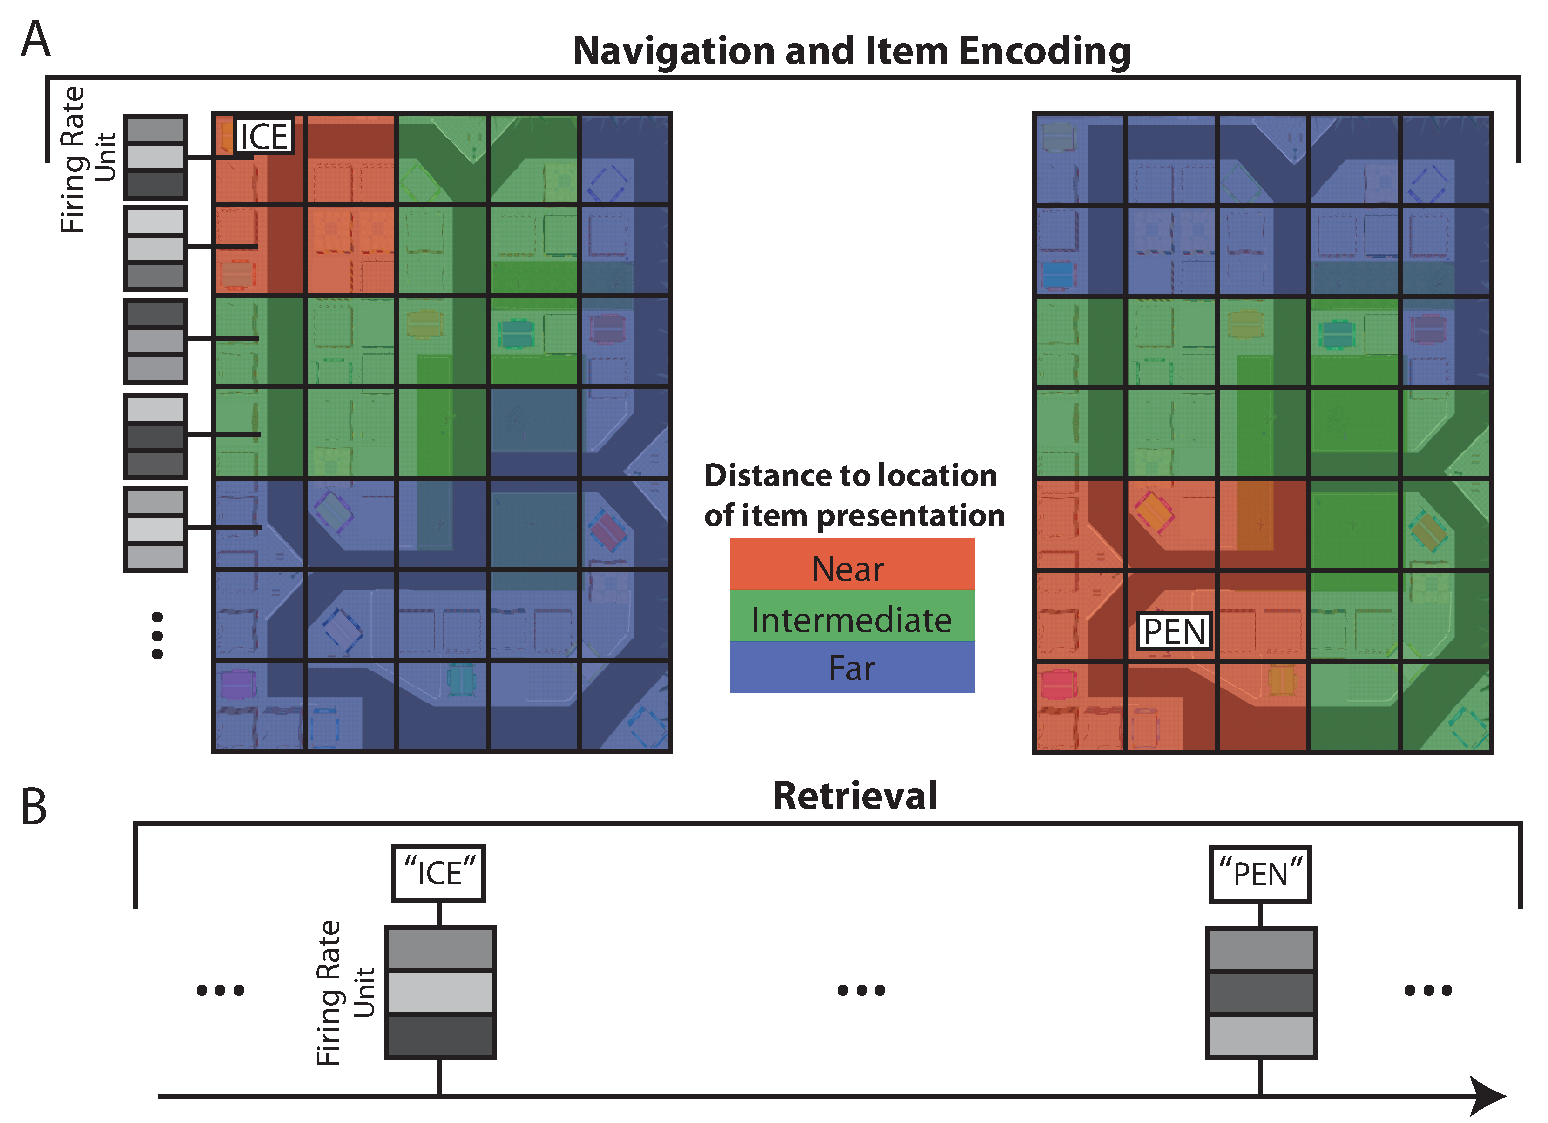
\includegraphics[width=.95\textwidth]{./tex/dboy/figs/methods}
  \caption[Spatial context reinstatement analysis method]{A schematic of the spatial context reinstatement via ensemble activity analysis. In these hypothetical examples, an item is presented to the subject in a particular sector of the town, as indicated in Panel A.  Red shading indicates sectors considered spatially close the presentation location, green shading indicates sectors considered spatially intermediate, and blue shading indicates sectors considered spatially far. In a given session, the mean firing rate of all identified place-responsive cells was calculated separately for each sector (represented visually by the shaded grey boxes).  During retrieval of the same item, the mean activity of the place-responsive cells was calculated.  \textbf{A.} Two examples of the spatial binning of the environment. Left: the spatial binning of the environment if an item (``Ice'') was presented in the location indicated. Right: the spatial binning of the environment if an item (``Pen'') was presented in the location indicated.  \textbf{B.} In the retrieval period, the mean place-responsive cell firing rate during each item recall is calculated and compared the navigation activity (recall of ``Ice'' uses the spatial binning shown in panel A Left and recall of ``Pen'' uses the spatial binning shown in panel A Right).}
\label{fig:methods}
\end{figure}

 \begin{figure}
\centering
  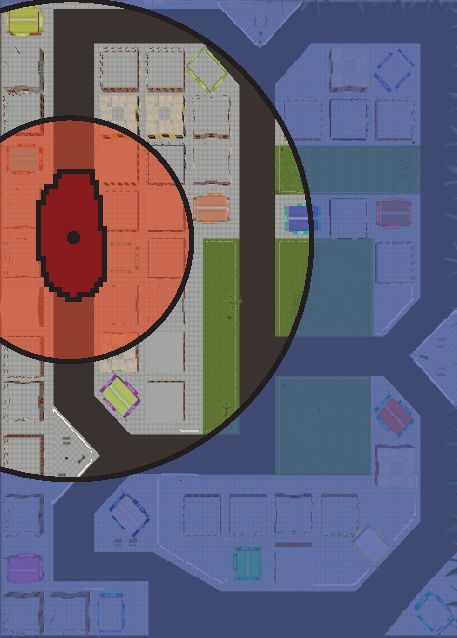
\includegraphics[width=.6\textwidth]{./tex/dboy/figs/firing_rate_method}
  \caption[Spatial context reinstatement via individual cell firing rate analysis method]{A visual representation of the spatial context reinstatement via individual cell firing rate analysis. The dark red area represents a cell's place field, and the dot in the middle of the place field represents the center of mass.  Items delivered to the store falling within the transparent red circle would be considered near to the place field. Items delivered to stores falling within the transparent blue circle would be considered far from the place field. The radii of the circles emanating from the center of mass are determined by the length of the major axis of the place field (1 times the major axis and 2 times the major axis for near and far, respectively).}
\label{fig:fr_by_cond_methods}
\end{figure}

 \begin{figure}
\centering
  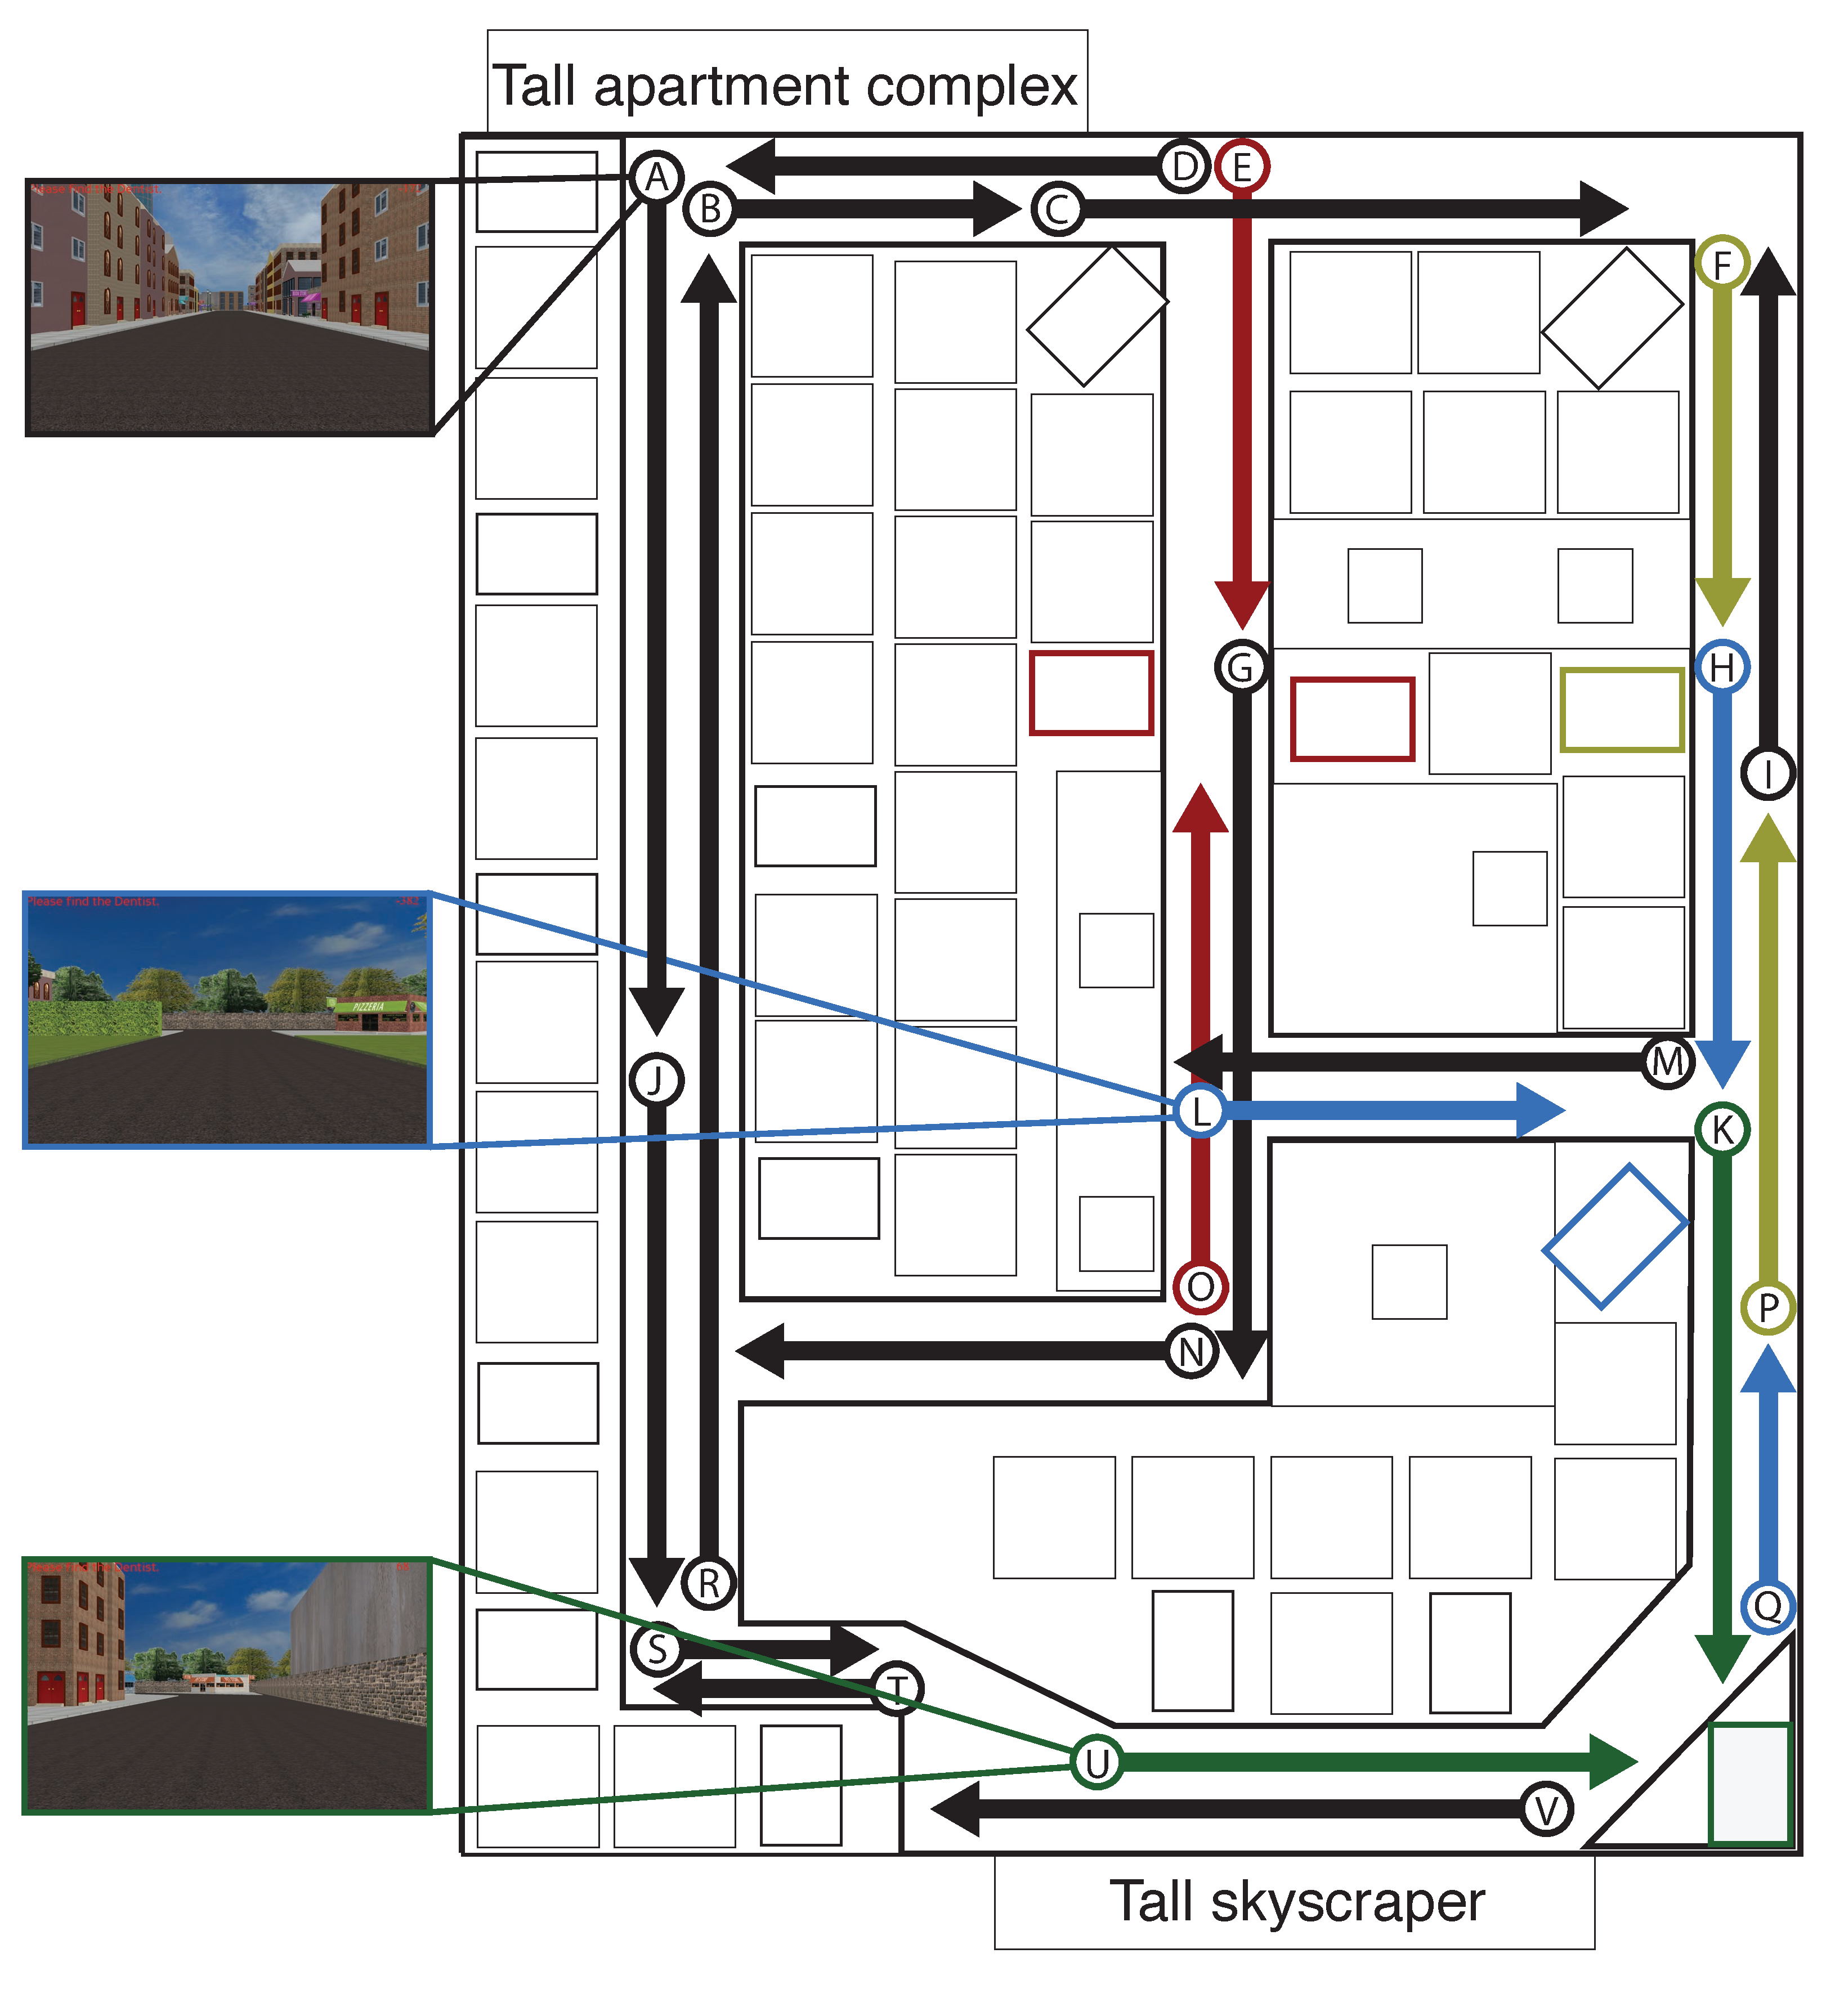
\includegraphics[width=.7\textheight]{./tex/dboy/figs/viewSmall}
  \caption[View-responsive cell analysis method]{A visual representation of how the environment was divided into regions for the view-responsive cell analysis. Each arrow represents the area of the town and direction of travel for its respective region. Arrows with the same color (excluding black arrows, which are all distinct regions) shared a primary landmark, and thus were treated in the analysis as the same region (colored rectangles represent the landmark shared among these regions). For illustrative purposes, screenshots of three of the regions are shown on the left (regions \emph{A}, \emph{L}, and \emph{U}, taken at the beginning (tail end) of their respective arrows. Note that the field of view during navigation was 60$^\circ$, thus objects and landmarks immediately to sides of the current location are not visible.}
\label{fig:view_methods}
\end{figure}

\clearpage
\section{Supplemental Tables}
\begin{table}[ph]
\centering
%  \begin{scriptsize}
% \begin{tabular}{|c|C{.8cm}|C{1.3cm}|C{1cm}|C{1cm}|C{1cm}|C{.8cm}|C{.8cm}|C{1cm}|C{.8cm}|C{.8cm}|}
 \begin{tabular}{|ccc|ccccc||c|}

\multicolumn{3}{c|}{} & \multicolumn{5}{|c||}{Region} & \multicolumn{1}{c}{}\\\hline
      Subject $\#$ & Session & Trials & H & A & EC & PHG & ANT & Totals\\\hline
      \multirow{3}{*}{1} & 1 & 1 & 4 of 16 & 2 of 5 & 5 of 8 & 0 of 0 & 0 of 0 & 11 of 29\\
      & 2 & 1 & 5 of 26 & 0 of 4 & 5 of 11 & 0 of 0 & 0 of 0 & 10 of 41\\
      & 3 & 2 & 6 of 17 & 0 of 5 & 1 of 8 & 0 of 0 & 0 of 0 & 7 of 30\\\hline
      \multirow{3}{*}{2} & 1 & 1 & 6 of 8 & 0 of 0 & 2 of 9 & 1 of 7 & 0 of 0 & 9 of 24\\
      & 2 & 3 & 0 of 0 & 0 of 0 & 4 of 11 & 0 of 7 & 0 of 0 & 4 of 18\\
      & 3 & 2 & 1 of 4 & 0 of 0 & 1 of 8 & 0 of 6 & 0 of 0 & 2 of 18\\\hline
      \multirow{3}{*}{3} & 1 & 3 & 6 of 17 & 3 of 7 & 0 of 0 & 0 of 0 & 0 of 0 & 9 of 24\\
      & 2 & 3 & 4 of 10 & 1 of 4 & 0 of 0 & 0 of 0 & 0 of 0 & 5 of 14\\
      & 3 & 3 & 7 of 17 & 3 of 8 & 0 of 0 & 0 of 0 & 0 of 0 & 10 of 25\\\hline
      \multirow{2}{*}{4} & 1 & 6 & 1 of 4 & 5 of 9 & 0 of 0 & 0 of 0 & 1 of 4 & 7 of 17\\
      & 2 & 8 & 0 of 1 & 3 of 7 & 0 of 0 & 0 of 0 & 1 of 2 & 4 of 10\\\hline
      5 & 1 & 6 & 1 of 12 & 0 of 8 & 1 of 8 & 0 of 0 & 0 of 0 & 2 of 28\\\hline
      \multirow{2}{*}{6} & 1 & 4 & 1 of 10 & 0 of 2 & 0 of 0 & 0 of 0 & 1 of 14 & 2 of 26\\
      & 2 & 4 & 1 of 13 & 0 of 0 & 0 of 0 & 0 of 0 & 3 of 11 & 4 of 24\\\hline
      \multirow{2}{*}{7}  & 1 & 10 & 1 of 17 & 0 of 0 & 3 of 7 & 0 of 0 & 0 of 0 & 4 of 24\\
      & 2 & 8 & 4 of 17 & 0 of 0 & 1 of 2 & 0 of 0 & 0 of 0 & 5 of 19\\
\hline
\multicolumn{3}{c|}{Totals} & 48 of 189 & 17 of 59 & 23 of 72 & 1 of 20 & 6 of 31 & \multicolumn{1}{c}{95 of 371}\\
    \end{tabular}
%  \end{scriptsize}
  \caption[Summary of place-responsive cells]{Summary of place-responsive cell counts across subjects. The table shows the total number of cells and the total number of place-responsive cells for each recording session, aggregated by brain region (H: hippocampus, A: amygdala, EC: entorhinal cortex, PHG: parahippocampal gyrus, ANT: localization accuracy limited to anterior MTL). Sessions with less than four place-responsive cells were excluded from reinstatement analyses. Though session 1 of subject 1 had 11 identified place-responsive cells, it was excluded from the reinstatement analyses due to not having any valid recalls.}
\label{tab:counts}
\end{table}

\clearpage



\begin{table}[ph]
\centering
%  \begin{scriptsize}
% \begin{tabular}{|c|C{.8cm}|C{1.3cm}|C{1cm}|C{1cm}|C{1cm}|C{.8cm}|C{.8cm}|C{1cm}|C{.8cm}|C{.8cm}|}
 \begin{tabular}{|c|lcccc|}
\hline
Subject $\#$ & Region & $\#$ Cells & FR (Hz) & In Field FR (Hz) & Field Size\\\hline

\multirow{4}{*}{1} & Amygdala & 2 of 14  & 0.18 & 0.54 & 2.64 \\ 
 & EC & 11 of 27  & 2.09 & 3.60 & 2.59 \\ 
 & Hipp Body & 8 of 31  & 0.82 & 2.94 & 2.76 \\ 
 & Hipp Head & 7 of 28  & 0.32 & 0.89 & 2.77 \\ \hline
\multirow{3}{*}{2} & EC & 7 of 28  & 1.82 & 4.53 & 2.68 \\ 
 & Hipp Body & 7 of 12  & 0.37 & 5.97 & 3.26 \\ 
 & PHG & 1 of 20  & 0.39 & 4.48 & 5.43 \\ \hline
\multirow{2}{*}{3} & Amygdala & 7 of 19  & 0.63 & 2.38 & 2.47 \\ 
 & Hipp Head & 17 of 44  & 1.28 & 2.62 & 2.41 \\ \hline
\multirow{3}{*}{4} & Amygdala & 8 of 16  & 4.07 & 5.64 & 2.43 \\ 
 & Hipp Head & 1 of 5  & 0.23 & 0.82 & 2.37 \\ 
 & Anterior MTL & 2 of 6  & 0.35 & 1.22 & 2.46 \\ \hline
\multirow{3}{*}{5} & Amygdala & 0 of 8  & - & - & - \\ 
 & EC & 1 of 8  & 0.05 & 0.60 & 2.35 \\ 
 & Hipp Head & 1 of 12  & 0.27 & 1.12 & 2.20 \\ \hline
\multirow{4}{*}{6} & Amygdala & 0 of 2  & - & - & - \\  
 & Hipp Head & 2 of 15  & 0.15 & 1.60 & 3.01 \\ 
 & Hipp Tail & 0 of 8  & - & - & - \\ 
 & Anterior MTL & 4 of 25  & 7.78 & 9.71 & 2.52 \\ \hline
\multirow{3}{*}{7} & EC & 4 of 9  & 1.31 & 2.32 & 2.90 \\ 
 & Hipp Body & 4 of 21  & 6.13 & 7.87 & 2.52 \\ 
 & Hipp Head & 1 of 13  & 3.89 & 5.38 & 2.37 \\ 
\hline
    \end{tabular}
%  \end{scriptsize}
  \caption[Place-responsive cells characteristics]{Place-responsive cells characteristics by subject and region. For each subject, only regions in which cells were recorded are included. The column ``$\#$ Cells'' shows the number of place-responsive cells recorded, out of the total number of cells. The column ``FR (Hz)'' shows the average firing rate within a region  for all movement epochs during the task, regardless of location in the virtual environment.  The column ``In Field FR (Hz)'' shows the average firing rate within a region within the cells' place fields. The column ``Field Size'' shows the average size of the place fields within a region as a percentage of the traversable area of the virtual environment.}
\label{tab:counts}
\end{table}




\clearpage

% \bibliographystyle{Science}



    % CHAPTER 3: Miller et al., 2015
    \chapter{Repeating spatial activations in human entorhinal cortex}
    \begin{quotation}
    \singlespacing
    \noindent Jonathan F. Miller, Itzhak Fried, Nanthia Suthana, \& Joshua Jacobs \\ \textit{Current Biology}
    \end{quotation}
     

  
  
\section{Summary}

The ability to remember and navigate spatial environments is critical for everyday life. A primary mechanism by which the brain represents space is through hippocampal place cells, which indicate when an animal is at a particular location \citep{OKeeDost71}. An important issue is understanding how the hippocampal place-cell network represents specific properties of the environment, such as signifying that a particular position is near a doorway or that another position is near the end of a corridor. The entorhinal cortex (EC), as the main input to the hippocampus, may play a key role in coding these properties because it contains neurons that activate at multiple related positions per environment \cite{FranEtal00,HaftEtal05,DerdEtal09,SolsEtal08,BjerEtal14}.  We examined the diversity of spatial coding across the human medial temporal lobe by recording neuronal activity during virtual navigation of an environment containing four similar paths. Neurosurgical patients performed this task as we recorded from implanted microelectrodes, allowing us to compare the human neuronal representation of space with that of animals. EC neurons activated in a repeating manner across the environment, with individual cells spiking at the same relative location across multiple paths. This finding indicates that EC cells represent non-specific information about location relative to an environment's geometry, unlike hippocampal place cells, which activate at particular random locations. Given that spatial navigation is considered to be a model of how the brain supports non-spatial episodic memory \cite{EichLipt08,BirdBurg08,Hass12,BuzsMose13}, these findings suggest that EC neuronal activity is used by the hippocampus to represent the properties of different memory episodes \cite{FranEtal00,BuckEtal04}.




\section{Results}
We recorded 1,329 single neurons in various brain regions from 13 neurosurgical patients performing a virtual-navigation task.  Patients were instructed to learn an environment's layout and navigate between six destination ``stores''  as rapidly and accurately as possible. This environment was a square track (see Figure~\ref{fig:behaviorCurrBio}A), which limited the patients' navigation path to particular regions of the environment. Navigation errors decreased across trials of the task (Figure~\ref{fig:behaviorCurrBio}B), indicating that patients successfully learned the environment's layout.
  

\begin{figure} \centering 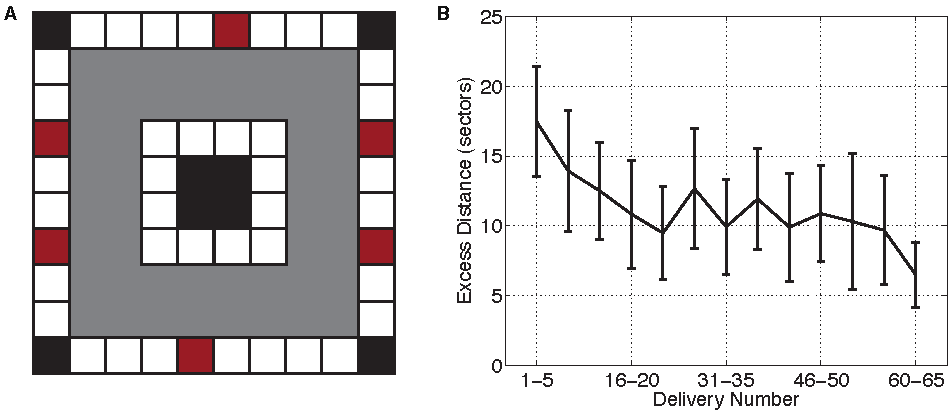
\includegraphics[width=.9\textwidth]{./tex/linearGrids/figs/Figure1} \caption[Behavioral task and performance]{\textbf{Behavioral task and performance.} \textbf{(A)} An overhead schematic of the layout of the virtual environment. Red squares represent locations of the destination stores and white square are non-store buildings. Gray shading indicates regions of the environment where the patient could travel. \textbf{(B)} Subject average task performance as a function of delivery trial number. Performance is measured as the excess number of sectors traveled when searching for a destination store, compared to an ideal path. Error bars are 95\% confidence intervals. See also Figure~\ref{fig:subOcc}.} \label{fig:behaviorCurrBio}
\end{figure}


Our main objective was to characterize how the spiking of individual neurons varied to represent  the patient's virtual spatial location. For each cell, we computed firing rate maps corresponding to the cell's mean rate of spiking as a function of the current  virtual location. A previous analysis of this dataset \cite{JacoEtal10} revealed  many \emph{path cells}, which coded for whether the participant was traveling clockwise or counterclockwise around the track. Thus, we computed firing rate maps separately for movements in clockwise and counterclockwise directions. We  calculated these maps  in a smoothed manner, as well as in a discretized manner that binned the patients' location into one of 25 sectors on each side of the track.

Next, we identified cells that significantly varied their firing rate according to the patient's virtual location. We used a one-way ANOVA as a screening procedure to identify individual neurons whose firing rates varied in response to the current sector of the environment. According to this measure, 313  cells (23.5\%) were responsive to the location, a percentage that is in line with previous single-cell studies of human virtual navigation \cite{EkstEtal03,JacoEtal10,JacoEtal13}. Our subsequent analyses focused on more precisely characterizing the activity of these cells.


A distinctive feature of some location-responsive cells in rodents is that they activate at multiple  spatial locations that are related to each other, such as positions just before or after a curve \cite{FranEtal00}, locations at particular distances from borders \cite{SolsEtal08,DerdEtal09,BjerEtal14}, or spots associated with particular landmarks \cite{HargEtal05,TsaoEtal13}.  We sought to identify analogous  types of representations in humans by searching for cells that exhibited significant \emph{path equivalence} across distinct sections of the virtual environment \cite{FranEtal00}.  We computed the path-equivalence coefficient for each cell, which is a measure of the similarity of the cell's firing activity across two or more corridors (see \emph{Experimental Procedures}).  A cell that exhibited significant path equivalence is one that activated at the same relative position on multiple sides, such as a cell that spiked when a person was passing through the midpoint of any of the four paths.  Of the 313 location-responsive cells, 30 (9.6\%) exhibited significant path-equivalent firing patterns ($p<0.001$).


\begin{figure}[t]
\centering
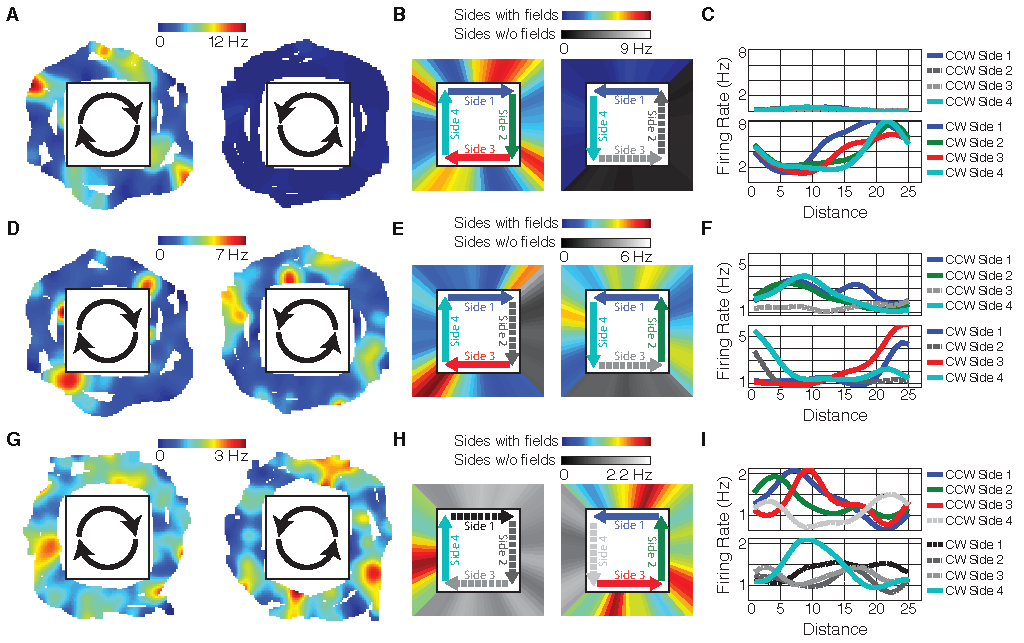
\includegraphics[width=.99\textwidth]{./tex/linearGrids/figs/Figure2}
\caption[Path equivalent cell firing rate maps]{\textbf{Path equivalent cell firing rate maps.} \textbf{Top Row:} Activity of a cell in patient 2's entorhinal cortex. \textbf{(A)} Two dimensional firing rate map for epochs of clockwise (left) and counterclockwise (right) movement. \textbf{(B)} Linearized firing rate maps (smoothed with a 12-pt window) for epochs of clockwise (left) and counterclockwise (right) movement. Sides with regions of significantly elevated firing are shown in color, and sides without significant activations are in grayscale. \textbf{(C)} Firing rate as a function of distance from the beginning of the side, plotted separately for each side of the environment and for clockwise (bottom) and counterclockwise (top) directions. \textbf{Middle Row:} Activity of a cell in patient 2's  entorhinal cortex. \textbf{Bottom Row:} Activity of a cell in patient 5's cingulate cortex. See also Figure~\ref{fig:subDots}.}
\label{fig:firingExamples}
\end{figure}

Three example path equivalent cells are shown in Figure~\ref{fig:firingExamples}. Figure~\ref{fig:firingExamples}A--C highlights one cell in the EC that activated consistently as the patient approached the end of each corridor during clockwise movement. Figure~\ref{fig:firingExamples}D--F shows a different cell in the EC that activated at similar locations across multiple corridors, with the locations of activations shifting between clockwise and counterclockwise movements. Figure~\ref{fig:firingExamples}G--I illustrates a cell from cingulate cortex that activated near the beginning of multiple corridors during counterclockwise movement. Additional example cells are shown in Figure~\ref{fig:otherExamples}.

We found significant levels of path-equivalent cells in only two regions: the entorhinal cortex and the cingulate cortex (Figure~\ref{fig:population}A).  The magnitude of individual cells' path-equivalent firing was greater in EC compared to cingulate cortex, as indicated by the fact that the mean path-equivalence coefficient for EC path-equivalent cells (0.92) was greater than for path-equivalent cells in cingulate cortex (0.49; $p<.05$, rank-sum test). We specifically compared the level of path-equivalent activity between the hippocampus and its main input, the entorhinal cortex, and found that the entorhinal cortex contained more path-equivalent cells than the hippocampus ($p<0.05$, post-hoc $\chi^2$ test). This difference in the prevalence of path-equivalent cells cannot be attributed to a difference in the stability of the spatial coding between EC and hippocampus, as these two regions did not differ in the percentage of location sensitive cells that were stable over time (45\% EC vs 53\% hippocampus, n.s.).  Prior research suggested functional differences across regions within the entorhinal cortex \cite{HaftEtal05,HargEtal05,BrunEtal08a}.  However, we did not find any difference in the proportion of path-equivalent cells between neurons located in the posterior vs.\ anterior EC, lateral vs.\ medial, or superior vs.\ inferior positions ($\chi^2$ tests, all $p$'s$ > 0.1$).

\begin{figure}[t]
\centering 
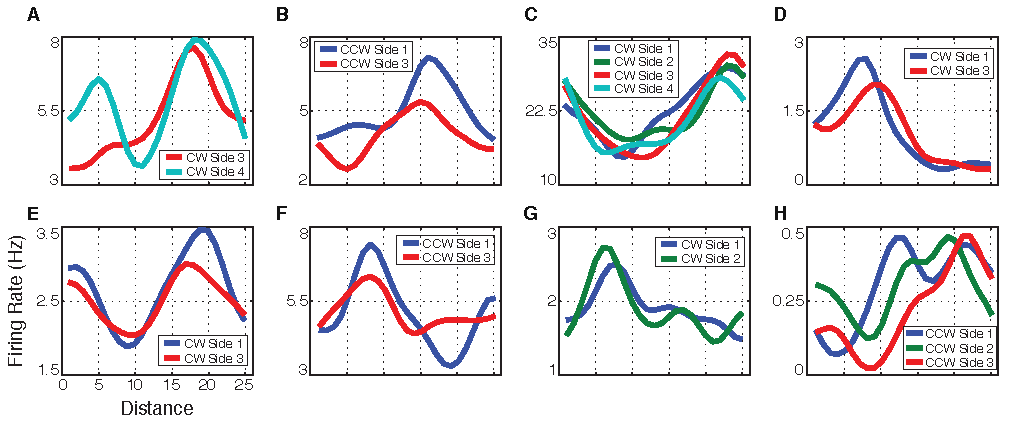
\includegraphics[width=.99\textwidth]{./tex/linearGrids/figs/Figure3}
\caption[Examples of path equivalent cells]{\textbf{Examples of path equivalent cells.} \textbf{(A)} A cell from patient 1's cingulate cortex during clockwise movement. \textbf{(B)} A cell from patient 2's entorhinal cortex during counterclockwise movement. \textbf{(C)} A cell from patient 2s entorhinal cortex during clockwise movement. \textbf{(D)} A cell from patient 5's entorhinal cortex during clockwise movement. \textbf{(E)} A cell from patient 10's parahippocampal gyrus during clockwise movement. \textbf{(F)} A cell from patient 12's entorhinal cortex during counterclockwise movement. \textbf{(G)} A cell from patient 13's hippocampus during clockwise movement. \textbf{(H)} A cell from patient 13's hippocampus during counterclockwise movement. See Figure~\ref{fig:subOtherEx} for additional examples.} \label{fig:otherExamples}
\end{figure}


The path-equivalence measure we employed is sensitive to the overall shape of a cell's firing pattern.  Thus, this measure could be influenced by cells with diffuse firing patterns \cite{QuirEtal92} rather than the spatially precise activations  of conventional place or grid cells.  To verify that the pattern of path-equivalent cells we observed was driven by the locations of peak spatial activations, we directly tested whether the relative locations of peak firing  (place fields) were maintained across the sides of the environment. We identified each cell's place fields and then computed, for each cell, the percent of pairs of corridors of the environment where the relative locations of the place fields overlapped by at least 50\% (Figure~\ref{fig:population}B).  This analysis supports  the finding that the EC plays a particular role in path equivalence because cells in EC had the greatest percent of corridors where place fields were located at the same relative location. Across all cells with place fields on two or more corridors in the EC, 40\% of the possible corridor pairs had fields in overlapping locations. This is significantly more than the  22\% of corridor pairs for cells in cingulate cortex ($p<.05$, ranksum test). If we restrict this analysis to only the previously identified path-equivalent cells, the difference is more pronounced (87\% compared to 47\%).


\begin{figure}[t]
\centering
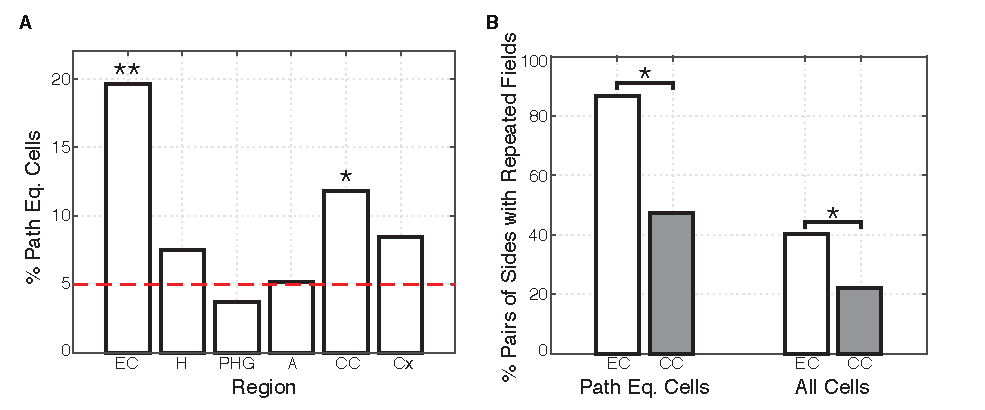
\includegraphics[width=.99\textwidth]{./tex/linearGrids/figs/Figure4}
\caption[Population measurements]{\textbf{Population measurements.}  \textbf{(A)} Regional distribution of \emph{path-equivalent cells}, which are location-responsive cells that have correlated responses across multiple corridors in the environment. EC: entorhinal cortex; H: hippocampus; PHG: parahippocampal gyrus; A: amygdala; CC: cingulate cortex; Cx: frontal/lateral-temporal cortex. \textbf{(B)} The percent of corridor pairs with place fields at the same relative locations.  This measure is computed by identifying each cell with place fields on at least two corridors and measuring, across all pairs of corridors, how often place fields occur at the same relative location.  $**$ denotes $p<.0001$, $*$ denotes $p<.05$. See also Figure~\ref{fig:subSpikes} and Table~\ref{tab:countsCurrBio}.}
\label{fig:population}
\end{figure}

One possibility is that individual neurons do not represent particular locations but rather that these  signals actually encode distance traveled.  We compared the location- or distance-encoding hypotheses  by comparing the firing patterns of neurons that exhibited place fields during both clockwise and counterclockwise directions. For the 25 path-equivalent cells that met this criterion, we computed the correlation between the mean clockwise and counterclockwise firing patterns. We distinguished distance and location-based firing by computing this correlation two ways: with the firing rate vectors aligned by absolute location, and with the vectors ordered by distance along the direction of movement. A positive correlation in the first case indicates location coding, whereas a positive correlation in the second indicates distance coding. Of the path-equivalent cells analyzed, 11 (44\%) showed significant correlations. Of these 11, 8 showed distance coding  (e.g., Fig.~\ref{fig:firingExamples}I), 1 showed location coding, and 2 were ambiguous. This result supports the hypothesis that some path-equivalent cells  play a role in representing relative distance  ($p<.05$, $\chi^2$ test).


\section{Discussion}

We examined human single-neuron recordings during virtual navigation and found a set of location-responsive cells that exhibited repeated firing patterns across multiple related areas of an environment. The key feature of these path-equivalent cells is that they consistently activated at the same relative position across separate corridors.  This  is the first evidence in humans that individual cells  generalize features across multiple  settings.  By activating at multiple locations, these cells behave very differently from place cells, which activate at only one location per environment. Because path-equivalent cells are input to the hippocampus, it indicates that a critical function of the human hippocampus is to build distinctive neuronal representations from non-specific entorhinal input. An additional contribution of our work is showing that  humans exhibit clear spatially modulated neuronal firing in \emph{virtual} navigation, supporting the view that virtual and physical navigation are supported by some similar mechanisms, as previously  demonstrated in rodents in various brain structures \cite{AghaEtal14,HarvEtal09,RavaEtal13}.


Our demonstration of EC path-equivalent cells complements previous studies describing rodent neurons with repeating spatial firing patterns. One example is a study by \citet{DerdEtal09}, which measured the activity of entorhinal grid cells as rodents navigated a constrained track. During movement in one direction of a hairpin maze, grid cells activated to represent equally spaced groups of locations that were consistently positioned across multiple corridors. As that paper demonstrates, grid cells generally reset their grids at  entrances to individual corridors,  giving rise to the appearance of a repeating  pattern across different sections of the environment. Some of the cells in our study appear to exhibit a similar pattern, in which they reset their representation upon entering each corridor. This supports the view that the neural representation of space can be segmented by  entrances to different compartments  \cite{FranEtal00,SpieEtal13}.  

Our findings are also related to data from \citet{FranEtal00}, who reported path-equivalent cells in rodent EC.  The path-equivalent cells described in that study activated at analogous locations both within and across environments.  Although several aspects of our findings are similar to the cells from that study, one critical difference is that when path-equivalent cells activate, the rat always has the same compass-like absolute heading.  In contrast, for the path equivalent cells that we report, each activation corresponds to a circular heading and location within the environment.  In a previous study from this dataset, we reported \emph{path cells} that encoded direction in a circular manner such that they activated during either clockwise or counterclockwise movement \citep{JacoEtal10}.  Thus, one possibility is that the entorhinal representation of direction in humans can be transformed according to an environment's layout so that it may depart from a fixed compass-like orientation scheme. Although human EC path-equivalent share features with grid cells, it is premature to conclude that the data reported here are from grid cells.  As we demonstrate in Figure~\ref{fig:subDots}, owing to the four-way symmetry of our square environment, our data are not consistent with a grid cell that encoded the patient's position using a triangular coordinate system in two-dimensional space.  We could not test whether the cells in our dataset exhibit grids aligned  individual corridors \cite{DerdEtal09} because the length of each corridor was too short to observe a possible grid repetition.
 
As studies of rodent spatial navigation characterize the functional relationship between different brain regions, theories of hippocampal function are converging on the idea that rodent spatial navigation is a model for studying other aspects of cognition, including episodic memory \citep{EichEtal99,Buzs05,BuzsMose13,MoseMose13}. These theories share the idea that the representation of specific episodic memories can be considered analogous to the representation of locations by place cells. The role of the EC in this system may be to represent non-specific features of the behavioral setting \citep{HaftEtal05,SolsEtal08,SargEtal06,JacoEtal13,JacoEtal10} for encoding into specific memories (or locations) by the hippocampus \cite{NormORei03}. During navigation, EC neurons may  represent the attributes of a setting, with each cell activating at related   locations, as in our findings and in some earlier animal work  \cite{FranEtal00}.  To our knowledge, our findings are the first demonstration of this type of featural neuronal coding in the human EC (cf.\ Mormann et al., 2008 \cite{MormEtal08}). By demonstrating a key difference between hippocampal and entorhinal representations during navigation, our results support theoretical models regarding the diversity of information processing throughout the medial temporal lobe \cite{NormORei03,KnieEtal06,SolsEtal06}. 
 



\section{Experimental procedures}

\paragraph{Participants and Task Design.} The task design and methods for data acquisition are described in a previous study that examined this same dataset \citep{JacoEtal10}. All data analyses and results reported here are novel, although the prior study \citep{JacoEtal10} did qualitatively describe the activity of one cell we examined here. Thirteen patients undergoing surgical treatment for medication-resistant epilepsy participated in the study.  All surgeries were performed by I.F. and the research protocol was approved by the University of California, Los Angeles Institutional Review Board.  Patients played a 3D virtual navigation game on a laptop computer in their hospital room \citep{EkstEtal03,JacoEtal10,JacoKaha10,JacoEtal13}. The virtual environment consisted of six destination stores surrounding the perimeter of a square track, with the center of the environment obstructed by buildings (Figure~\ref{fig:behaviorCurrBio}A). On each delivery trial the patient transported a passenger to their requested store destination as accurately as possible.  After arrival at the destination, on-screen text displayed the name of the next randomly selected destination store.

\paragraph{Electrophysiology.}  We recorded spiking activity at 28--32~kHz using 40-$\mu$m platinum-–iridium microwire electrodes \citep{FrieEtal99} connected to a Neuralynx recording system. Nine microwires extended from the tip of each clinical depth electrode. Action potentials were manually isolated using spike shape, clustering of wavelet coefficients, and interspike intervals \citep{QuirEtal04}.  We localized the locations of individual electrodes by co-registering post-operative CT scans with pre-implant MRI images and standardizing to a normalized brain \cite{TalaTour88}.

\paragraph{Data Preprocessing.} We binned the firing rate of each cell into 100-ms epochs. We labeled each epoch with the patient's location and direction of travel (either clockwise or counterclockwise around the square path). With the exception of the firing-rate maps presented in Figure~\ref{fig:firingExamples}A,D,G, all data analyses were conducted after linearizing patients' location into 100 discrete sectors (25 per side) along the square path.

\paragraph{Data Analysis.}
For each cell, we computed a one-way ANOVA as a screening procedure to identify cells whose firing rate varied significantly according to environment sector, assessing significance with a shuffling procedure \cite{EkstEtal03}. 
To determine whether a cell displayed a similar firing patterns across multiple sides of the square track, we used a modified version of the path equivalence coefficient from Frank et al.\ \citep{FranEtal00}. The path equivalence coefficient is a measure of the degree to which a cell fires in similar relative locations on multiple trajectories. Only sides of the track that contained at least one region of three or greater contiguous sectors of elevated firing were included.  We define the path-equivalence coefficient as the median correlation between the firing rates of all pairs of included sides minus the median correlation between the firing rates of all pairs of included sides and shuffled sides:

\(median(corr(side_{i},side_{j})) ~~ - ~~ median(corr(side_{i},shuf_{j}))\)

where $side$ is the firing rate of the corresponding 25 sectors, $shuf$ is the firing rate of the corresponding 25 sectors shuffled as described below, and $i$ and $j$ range from 1 to the number of included sides. To determine the firing rate values of a  shuffled side, the corresponding  firing rate values for the first half of that side were reversed and then the values of the two halves were swapped (e.g., a path of locations   ``A..BC..D''  become ``C..DA..B''). Statistical significance was determined using a permutation procedure (see \emph{Supplemental Experimental Procedures}).

\section{Supplemental data}

\begin{figure}[bh]
\centering
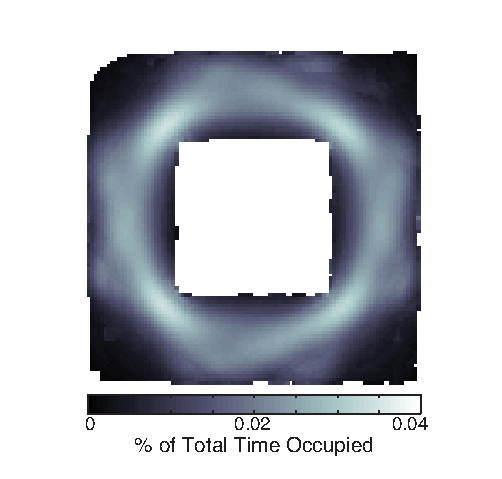
\includegraphics[width=.6\textwidth]{./tex/linearGrids/figs/supp_occupancy}
\caption[Average occupancy map]{Average occupancy map across all sessions. Brighter shading represents a greater amount of time spent in the region.}
% \end{center}
\label{fig:subOcc}
\end{figure}

\begin{figure}[bh]
\centering
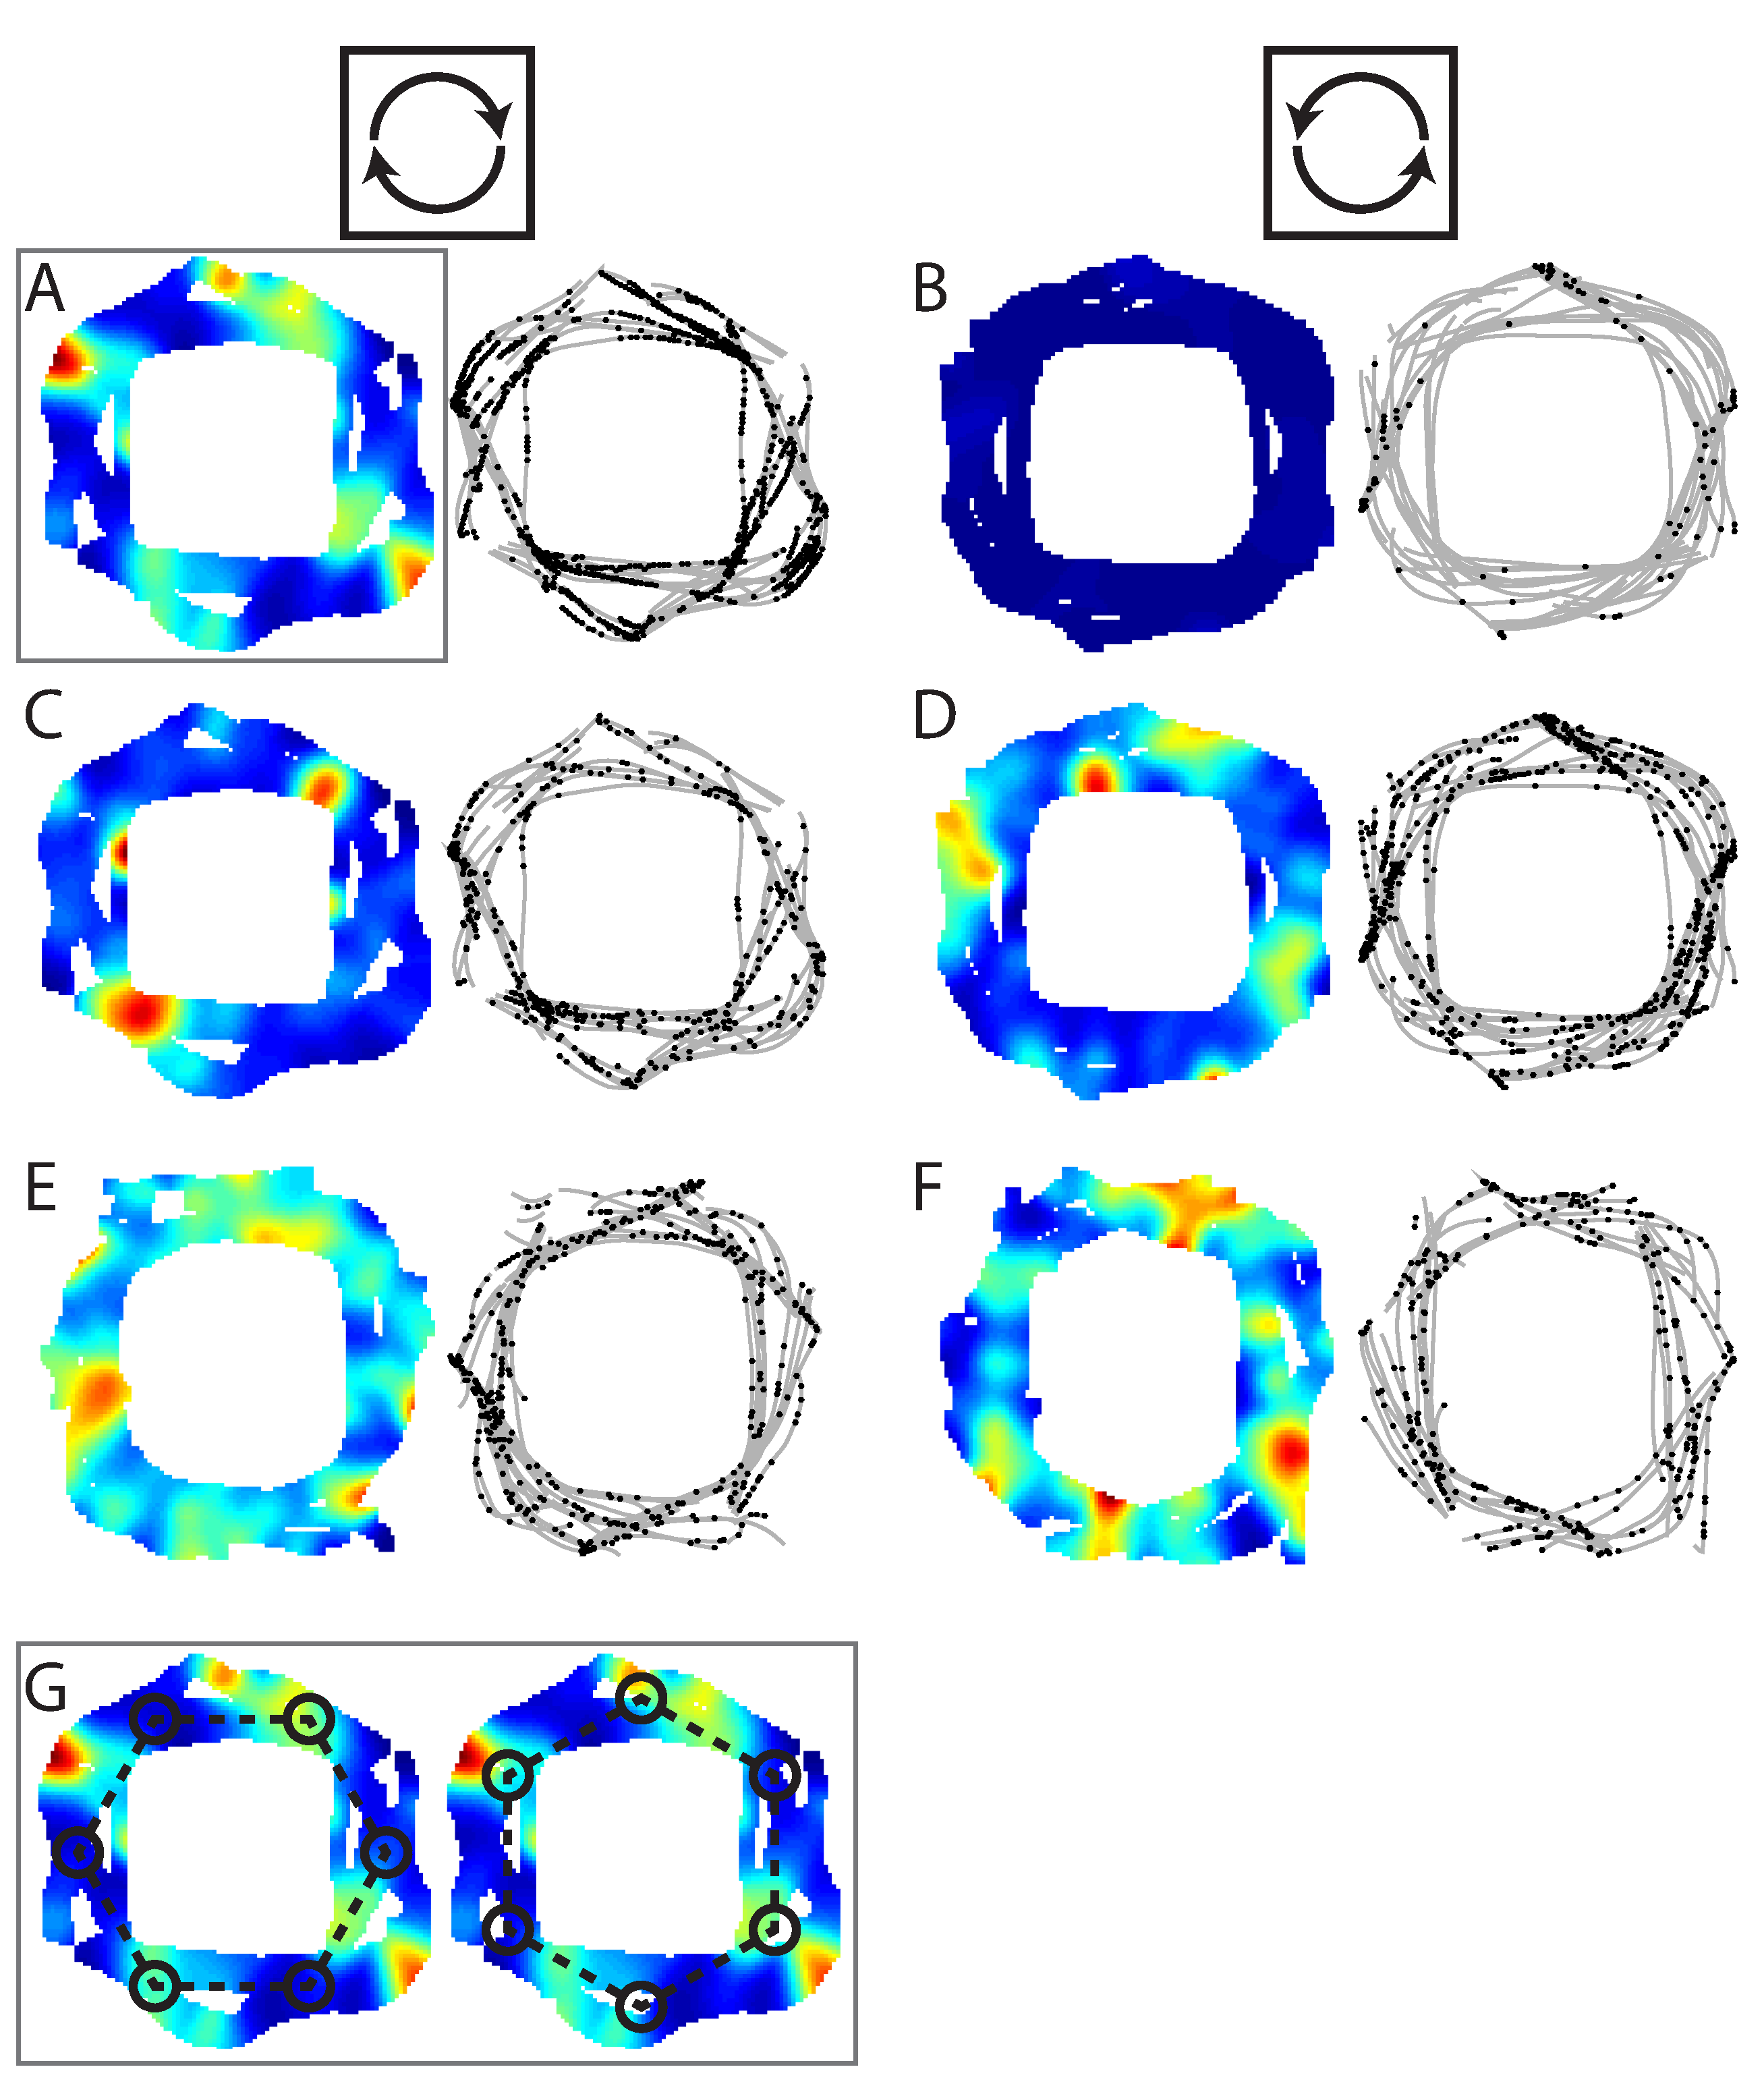
\includegraphics[width=.95\textwidth]{./tex/linearGrids/figs/supp_with_dots.pdf}
\caption[Firing rate maps and associated spiking activity]{\textbf{Firing rate maps and associated spiking activity. A-F. } The rate maps from Figure~\ref{fig:firingExamples} of the main text are replotted (left) along with the paths taken by the subject and locations where the cell fired, indicated by the gray lines and black dots, respectively (right). \emph{A,C,E:} Clockwise activity for the cells shown in Figure~\ref{fig:firingExamples}. \emph{B,D,F:} Counterclockwise activity for the cells shown in Figure~\ref{fig:firingExamples}. \textbf{G. } Firing rate map with an overlaid hexagon for a cell from patient 2's entorhinal cortex (as shown in panel A). The hexagon vertices do not closely fit the locations of the firing peaks, which suggests that our findings are not driven by a conventional grid cell that activates as if in an open arena. \emph{Left:} Unrotated hexagon. \emph{Right:} Hexagon rotated 30 degrees.}
% \end{center}
\label{fig:subDots}
\end{figure}

\clearpage
\begin{figure}[bh]
\centering
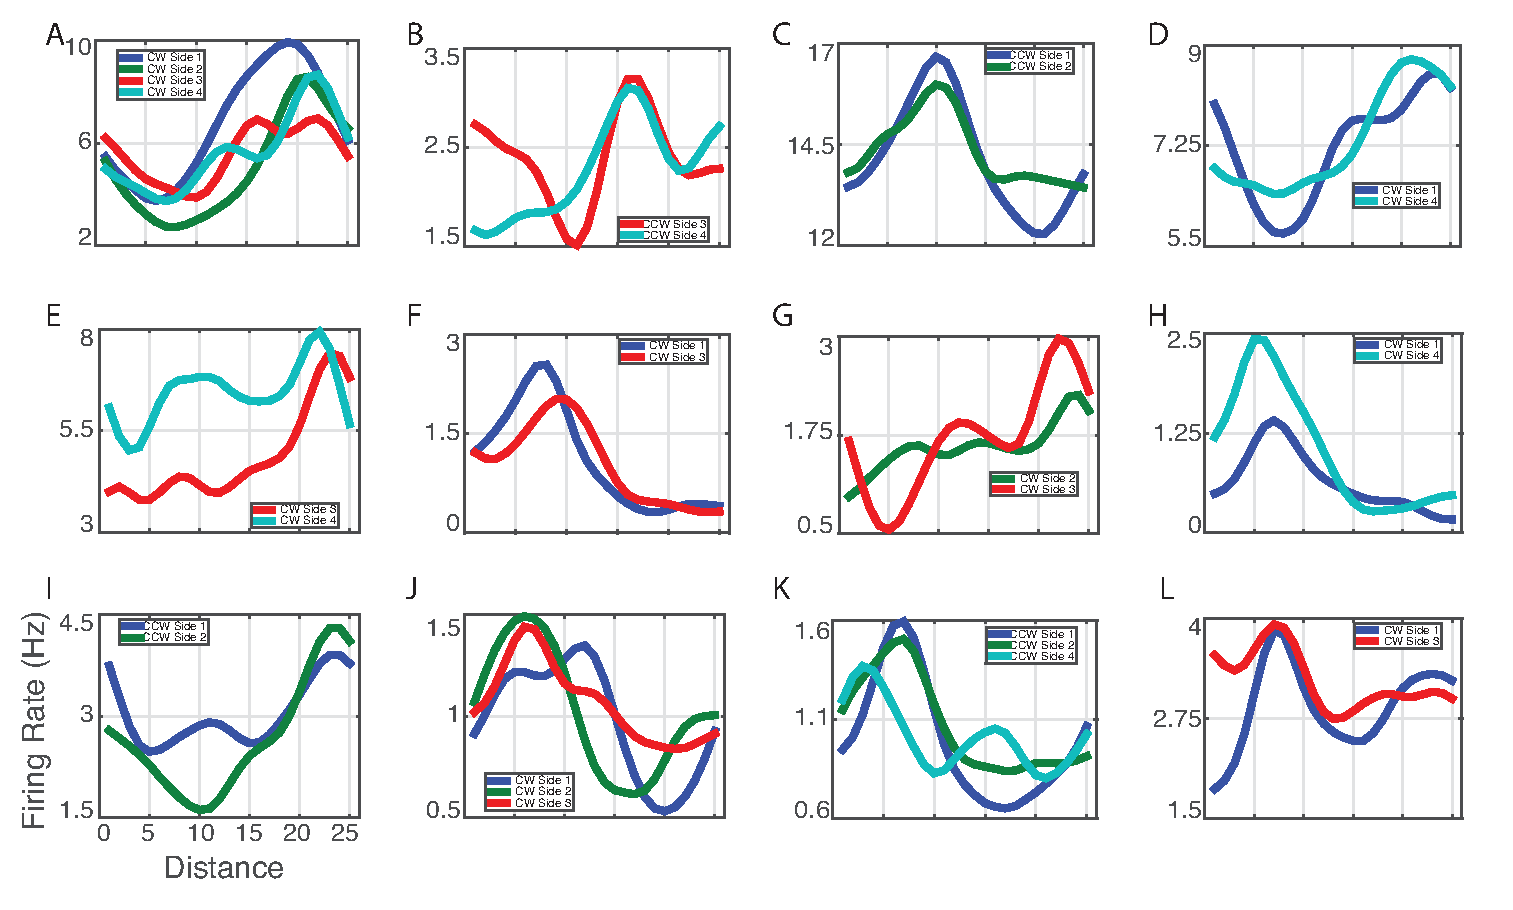
\includegraphics[width=1\textwidth]{./tex/linearGrids/figs/supp_extra_cells_large}
\caption[Additional examples of path equivalent (PE) cells]{\textbf{Additional examples of path equivalent (PE) cells.} \textbf{(A)} A PE cell from patient 2. \textbf{(B)} A PE cell from patient 3. \textbf{(C)} A PE cell from patient 3. \textbf{(D)} A PE cell from patient 4. \textbf{(E)} A PE cell from patient 4. \textbf{(F)} A PE cell from patient 5. \textbf{(G)} A PE cell from patient 6. \textbf{(H)} A PE cell from patient 6. \textbf{(I)}  A PE cell from patient 9. \textbf{(J--K)} One PE cell from patient 10 during two different directions of movement. \textbf{(L)}  A PE cell from patient 11.}
\label{fig:subOtherEx}
\end{figure}

	
\clearpage
\begin{figure}
\centering
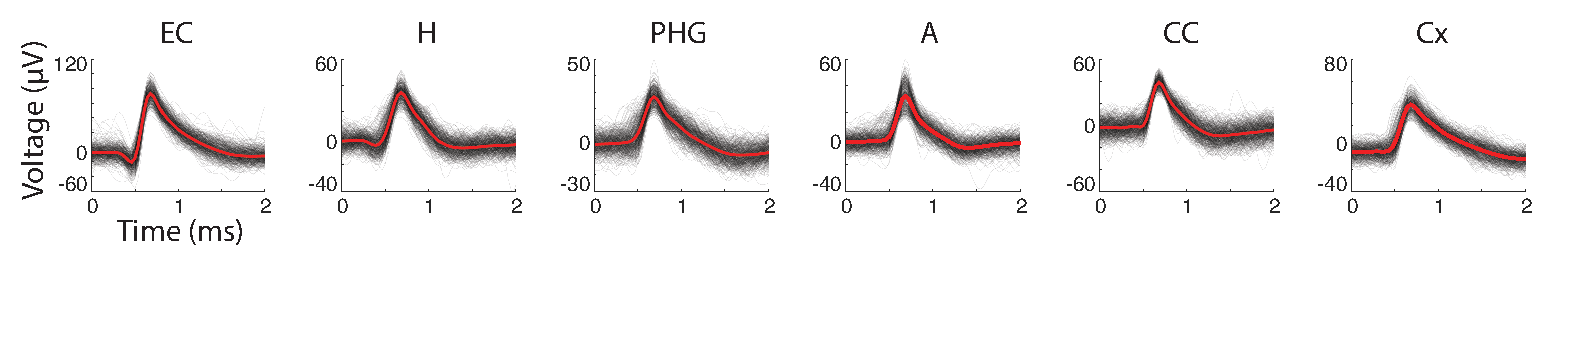
\includegraphics[width=.99\textwidth]{./tex/linearGrids/figs/waveforms}
\scriptsize	
 \begin{tabular}{|c|C{.5cm}|C{1cm}|C{.7cm}|C{.65cm}|C{1cm}|C{.8cm}|C{.8cm}|C{.8cm}|C{.8cm}|C{.8cm}|}
\hline
Region &Mean Firing Rate (Hz) &Firing Rate 5\%-95\% Range (Hz) &Mean Spike Amplitude ($\mu{}V$) &Background noise  ($\mu{}$V) &Mean False Positive (FP) Rate &FP below 10\% &FP below 20\% &Mean False Negative (FN) rate &FN below 10\% &FN below 20\%\\\hline
Entorhinal Cortex &4.0 &0.1-11.9 &44.8 &6.8 &3.7\% &91.1\% &95.6\% &4.2\% &88.6\% &94.9\%\\
Hippocampus &2.5 &0.1-10.3 &42.8 &6.7 &3.5\% &87.0\% &96.8\% &3.7\% &87.7\% &95.4\%\\
Parahippocampal Gyrus &2.0 &0.1-7.6 &36.8 &6.1 &2.0\% &95.7\% &97.9\% &2.6\% &94.7\% &95.7\%\\
Amygdala &2.7 &0.2-9.7 &51.9 &6.7 &7.6\% &77.8\% &88.3\% &7.5\% &77.1\% &88.3\%\\
Cingulate Cortex &4.1 &0.2-11.8 &45.0 &8.0 &6.7\% &79.1\% &89.8\% &7.4\% &76.7\% &86.4\%\\
Frontal/Temporal Cortex &3.2 &0.2-11.2 &42.3 &6.9 &5.0\% &80.3\% &92.2\% &5.1\% &80.3\% &91.9\%\\
\hline
\end{tabular}
\caption[Spike cluster characteristics]{Spike cluster characteristics. \textbf{Top:} Example spike waveforms from each brain region. Red line indicates the mean \textbf{Bottom:} Spike cluster isolation metrics. False-positive rate indicates the estimated percentage of spikes that were inappropriately designated as belonging to a given neuron.  False-negative rate indicates the percentage of spikes that were caused by a given neuron but were inappropriately labeled as belonging to neighboring neurons or noise. We compared the spike waveforms of path-equivalent cells with those of other neurons and did not find any differences in their mean amplitude (41~$\mu V$ for path-equivalent cells vs.\ 45~$\mu V$ for other cells; $p>0.35$, ranksum test) or in our false-positive or false-negative rates in  distinguishing their waveforms from neighboring cells ($p$'s$>0.1$, ranksum tests).}
% \end{center}
\label{fig:subSpikes}
\end{figure}	
	
\clearpage
\begin{table}
	\centering
	\small
\begin{tabular}{c|cccccc}
Subject \# & EC & H & PHG & A & CC & Cx\\\hline
1 &0 of 0 (0) &0 of 5 (12) &0 of 0 (0) &0 of 3 (20) &1 of 5 (18) &0 of 5 (28)\\
2 &5 of 18 (38) &0 of 6 (27) &0 of 0 (4) &0 of 0 (0) &0 of 9 (40) &0 of 10 (52)\\
3 &0 of 3 (12) &0 of 0 (3) &0 of 0 (0) &0 of 16 (74) &0 of 8 (14) &2 of 10 (47)\\
4 &1 of 6 (32) &1 of 11 (39) &0 of 0 (0) &1 of 5 (39) &2 of 13 (35) &0 of 0 (21)\\
5 &2 of 10 (34) &0 of 7 (45) &0 of 0 (0) &0 of 0 (0) &2 of 7 (38) &0 of 8 (51)\\
6 &1 of 9 (24) &0 of 0 (0) &0 of 0 (0) &1 of 2 (13) &1 of 5 (37) &1 of 10 (32)\\
7 &0 of 0 (0) &0 of 5 (24) &0 of 3 (5) &0 of 7 (23) &0 of 2 (5) &0 of 5 (17)\\
8 &0 of 0 (0) &0 of 6 (39) &0 of 5 (27) &0 of 0 (1) &0 of 0 (0) &0 of 0 (7)\\
9 &0 of 0 (0) &0 of 2 (8) &0 of 0 (0) &0 of 1 (2) &0 of 0 (0) &1 of 3 (9)\\
10 &0 of 0 (0) &1 of 5 (15) &1 of 9 (24) &1 of 9 (28) &0 of 0 (0) &0 of 0 (6)\\
11 &0 of 0 (0) &0 of 6 (26) &0 of 3 (4) &0 of 4 (12) &0 of 2 (19) &1 of 3 (37)\\
12 &1 of 2 (8) &0 of 1 (12) &0 of 3 (22) &0 of 8 (40) &0 of 0 (0) &0 of 0 (0)\\
13 &0 of 3 (10) &3 of 13 (35) &0 of 4 (8) &0 of 3 (14) &0 of 0 (0) &0 of 5 (13)\\
\hline Total &10 of 51 (158) &5 of 67 (285) &1 of 27 (94) &3 of 58 (266) &6 of 51 (206) &5 of 59 (320)\\
\end{tabular}
\caption[Summary of path equivalent cells]{Summary of path equivalent cells by patient and brain region. Counts indicate the number of path equivalent cells out of the total number of location-responsive cells. Numbers in parentheses indicate the total number of cells recorded, regardless of whether a cell was location-responsive. EC: entorhinal cortex; H: hippocampus; PHG: parahippocampal gyrus; A: amygdala; CC: cingulate cortex; Cx: frontal/lateral-temporal  cortex.}
% \end{center}
\label{tab:countsCurrBio}
\end{table}


\section{Supplemental experimental procedures}

\paragraph{Participants.} The task design and methods for data acquisition were described in a previous study that examined this same dataset \citep{JacoEtal10}. In brief, thirteen patients undergoing surgical treatment for medication-resistant epilepsy participated in the study.  All surgeries were performed by I.F. and the research protocol was approved by the University of California, Los Angeles Institutional Review Board.  Our dataset is comprised of 35 individual testing sessions (30--50 minutes each), with each participant contributing between one and four sessions.  All data analyses and results reported here are novel, although the prior study \citep{JacoEtal10} did qualitatively describe the activity of one cell we examined here.

\paragraph{Behavioral Task.} Patients played a virtual navigation game  \citep{EkstEtal03,JacoEtal10,JacoEtal13} on a laptop computer in their hospital room. The virtual environment consisted of six destination stores surrounding the perimeter of a square track, with the center of the environment obstructed by buildings. Patients traveled either clockwise or counterclockwise around the track. Two stores each were located on the east and west walls (sides 2 and 4), and one store each was on the north and south walls (sides 1 and 3). The stores were all visually distinct. The patients navigated the environment using a game controller. On each delivery trial the patient transported a passenger to their requested store destination as accurately as possible.  After arrival at the destination, on-screen text displayed the name of the next randomly selected destination store.

\paragraph{Electrophysiology.}  We recorded spiking activity at 28--32~kHz using 40-$\mu$m platinum-–iridium microwire electrodes \citep{FrieEtal99} connected to a Neuralynx recording system. Nine microwires extended from the tip of each clinical depth electrode. The first eight wires were insulated except for their tip and were used to record action potentials. The ninth microwire had its insulation stripped for $\sim$1~cm and served as the voltage reference for the other  wires. Action potentials were manually isolated using spike shape, clustering of wavelet coefficients, and interspike intervals \citep{QuirEtal04}.  We localized the locations of individual electrodes by co-registering post-operative CT scans with pre-implant MRI images and standardizing to a normalized brain \cite{TalaTour88}.  Assessing  entorhinal subregions is an  area of ongoing research \cite{KhanEtal14}. The approach we used to localize within the EC was by performing median splits across extent of our EC electrodes in the lateral/medial, anterior/posterior, and ventral/dorsal axes. % localize individual electrodes  For each dimension, we found the minimum and maximum coordinate across all of our EC electrodes, and we classified each electrode based on half of the total range.


\paragraph{Data Preprocessing.} We binned the firing rate of each cell into 100-ms epochs. We labeled each epoch with the patient's location and direction of travel (either clockwise or counterclockwise around the square path). Following previous work on this dataset \cite{JacoEtal07,JacoEtal10}, epochs without movement and epochs where clockwise or counterclockwise direction was not defined (i.e., when facing towards or away from the center of the environment) were excluded from analysis. With the exception of the firing-rate maps presented in Figure~\ref{fig:firingExamples}A,D,G, all data analyses were conducted after linearizing patients' location along the square path.   


\paragraph{Environment Linearization.} We linearized the paths of the environment by mapping the angle of every (x,y)-coordinate pair into 1 of 100 sectors, with the width of each sector equal to 3.6$^{\circ}$. We used this angular binning scheme because patients' generally followed a circular path during navigation (Figure~\ref{fig:subOcc}). When viewed in an overhead map, a linearized location value of 1 corresponds to the top-left corner of the environment. Values increase in a clockwise direction around the square path (thus, sectors 1--25 correspond to the top corridor, sectors 25--50 to the right, sectors 51--75 to the bottom, and sectors 76--100 to the left). After linearizing the location, we computed linearized firing rate maps separately for all epochs of clockwise movement and all epochs of counterclockwise movement. Linear firing rate maps were circularly convolved with a 6-sector gaussian window before data analyses.

\paragraph{Location-responsive cells.}
For each cell, we computed a one-way ANOVA as a screening procedure to identify cells whose firing rate varied significantly according to environment sector \cite{EkstEtal03}.  We separately validated (data not shown) that the outcome of this ANOVA  approach is very similar to the information theoretic approaches used by previous studies for this purpose  \cite{MarkEtal94}.  We created a distribution of 1000 p-values, each of which was the result of performing the ANOVA on shuffled firing rate maps, whereby the firing rate of the cell was circularly shifted by a random amount relative to the behavioral epochs. In order for a cell to be considered location-responsive, the p-value resulting from the unshuffled data must have been less than 900 of the p-values calculated using the randomly time-shifted data. We performed these calculations separately for epochs of clockwise and epochs of counterclockwise travel. A cell was considered spatially responsive if the true p-value met this criteria for either direction of travel.  Note that this screening ANOVA merely identifies cells whose firing rates vary systematically according to  location, which  is not the same as identifying bona fide place cells, as was performed on this dataset by Jacobs et al.\ (2010).

%
% In addition to the ANOVA, we report the results of an information-theory approach to identify spatially responsive cells \cite{MarkEtal94}, following the formula:
%
% \(information~content = \Sigma P_{i}(R_{i}/R)log_{2}(R_{i}/R)\)
%
% where $i$ is the sector number, $P_{i}$ is the probability of occupying sector $i$, $R_{i}$ is the firing rate of the cell in sector $i$, and $R$ is the mean firing rate of the cell. In order for a cell to be considered location-responsive using this information theory approach, the information content value must exceed 900 information content values calculated on shuffled firing rate maps. We performed these calculations separately for epochs of clockwise and epochs of counterclockwise travel.

\paragraph{Path Equivalent Cells.} To determine whether a cell displayed a similar firing patterns across multiple sides of the square track, we used a modified version of the path equivalence coefficient from Frank et al.\ \citep{FranEtal00}. The path equivalence coefficient is a measure of the degree to which a cell fires in similar relative locations on multiple trajectories. Only sides of the track that contained at least one region of three or greater contiguous sectors of elevated firing were included. In this way, our analyses focused on characterizing the specific locations where individual neurons activated, leaving future studies to examine the  important issue of why some cells show diminished firing in areas of certain environments. We define the path-equivalence coefficient as the median correlation between the firing rates of all pairs of included sides minus the median correlation between the firing rates of all pairs of included sides and shuffled sides:

\(median(corr(side_{i},side_{j})) ~~ - ~~ median(corr(side_{i},shuf_{j}))\)

where $side$ is the firing rate of the corresponding 25 sectors, $shuf$ is the firing rate of the corresponding 25 sectors shuffled as described below, and $i$ and $j$ range from 1 to the number of included sides. To determine the firing rate values of a  shuffled side, we followed the shuffling method of Frank et al.\ (2000) in which the firing rate values for the first half of the side were reversed and then the values of the two halves were swapped  (sequence ``A..BC..D''  would become ``C..DA..B'').

% To determine whether a cell's path equivalent coefficient value was greater than chance, for each cell we calculated 1000 path equivalent coefficients after randomly time-shifting the firing-rate measurements relative to behavior (as described above). If the true coefficient was greater than the 95\textsuperscript{th} percentile of coefficients calculated on shuffled data, then that coefficient was deemed to be significant at $p<0.05$. This procedure was done twice, one for clockwise movements and one for counterclockwise. If the path equivalent coefficient for either direction of movement was significant, then the cell was classified as a path equivalent cell.

To determine whether a cell's path equivalent coefficient value was greater than chance, we created a null distribution of 1000 path equivalent coefficients calculated on permuted data. For each permutation, we circularly shifted the 25 firing rate values of each included side by a random amount, independently for each included side, and recalculated the path equivalent coefficient. If the true coefficient was greater than the 95\textsuperscript{th} percentile of coefficients calculated on shuffled data, then that coefficient was deemed to be significant at $p<0.05$. This procedure was done twice, one for clockwise movements and one for counterclockwise. If the path equivalent coefficient for either direction of movement was significant, then the cell was classified as a path equivalent cell.


\paragraph{Place field analyses.}  We also used a shuffling procedure to identify the specific regions of the environment that exhibited significantly elevated firing rates (``place fields'') for each cell.  For a given cell and circular direction of travel we created a set of 1,000 shuffled firing rate maps, whereby the firing rate of the cell was circularly shifted by a random amount relative to the behavioral epochs. The firing rate within a sector was considered elevated if the activity from the unshuffled data was greater than the 90\textsuperscript{th} percentile of the firing rates for that sector from the shuffled data.

To quantify how often a single cell's place fields appeared at the same relative location on different sides of the path, we computed, for each cell, the degree of relative overlap of each pair of fields. We counted a pair of fields as overlapping if their relative position along each corridor overlapped by at least 50\%.  To ensure the results were unbiased for each cell, we limited the analysis to only sides with place fields, and divided the number of overlapping pairs by the total number of possible pairs (i.e., pairs of sides with place fields). Counts were combined across clockwise and counterclockwise directions. 

In the phenomenon of rate remapping, a cell distinguishes between different spatial representations via variations in the absolute firing rate levels  \cite{QuirEtal92,LeutEtal05,SingEtal10,AlleEtal12}.  We tested whether cells we observed exhibited a related phenomenon in which they varied their firing rates across different fields.  For each cell that exhibited two or more fields at the same relative location on different sides of the track (118 cells), we performed an ANOVA comparing the firings rates from when the patient occupied those fields. 8 of these cells (6.8\%) significantly varied their firing rates between related fields. This level is not significantly greater than chance (5\%) and thus not indicative of rate remapping.

The task's virtual environment exhibits reflective symmetry in that opposite corridors have similar store layouts.  There is one store on the east and west corridors and two stores on the north and south corridors (Figure~\ref{fig:behaviorCurrBio}A).  Given this layout, it was possible that a neural signal related to the quantity or location of nearby stores could masquerade as exhibiting path-equivalence between opposite walls of the environment.  We were interested in testing the possibility that path equivalence is related to the presence of nearby landmarks rather than the environment's overall spatial geometry.  For each cell with place fields on exactly two sides, we calculated how often the place fields were positioned on opposite versus neighboring sides.  This comparison was important because if two place fields appeared on opposite sides, then they could be driven by the identical store layouts between these areas. In contrast, if place fields were not related to stores, the percent of cells with fields on opposite sides would be at the chance level of 33\%. In line with this prediction, 32\% of the cells with two place fields had these fields positioned on opposite sides. We separately performed this analysis for cells from each brain region, with no region's percentage significantly differing from chance levels (all $p$'s$ > 0.1$).


\paragraph{Clockwise/Counterclockwise comparison.} For each path-equivalent cell, we classified the relationship between the cell's clockwise and counterclockwise firing patterns as either coding relative distance from the start of a corridor, coding absolute location, no relationship, or an ambiguous relationship. We only included cells with at least one place field in both directions of travel, and we only included corridors with  a place field. For each included cell, we performed two correlations. First, we correlated mean clockwise activity and mean counterclockwise activity directly such that a significant positive correlation indicates the encoding of location. We then correlated mean clockwise and mean counterclockwise activity with the counterclockwise vector  reversed, such that the first position in each vector follows the direction of movement to always represent the corridor's entry point. A significant positive correlation here indicates that a neuron encodes relative distance rather than location. If we observed a significant correlation in both cases (due, for example, to place fields in the middle of the corridors), we classified the relationship as ambiguous.





 
	
    % CHAPTER 4: Miller et al., 2015, in preparation  
    \chapter{TRAIN EXPERIMENT}
    \begin{quotation}
    \singlespacing
    \noindent Jonathan F. Miller \& Joshua Jacobs \\
    \end{quotation}	

    % CHAPTER 5: General discussion
    % !TEX root = ../thesis.tex
\chapter{General discussion}
\large

\section{Summary}

In this dissertation, I recorded intracranial brain activity as patients traveled through carefully designed 3D virtual environments in order to investigate the neural signals related to spatial navigation and memory function. My work shows that the neural mechanisms responsible for representing external space are also involved in the storage and retrieval of episodic memories, helping to reconcile how the hippocampus and medial temporal lobe (MTL) can simultaneously be vital for both navigation and declarative memory abilities. I have also advanced our understanding of exactly how space is coded in the human brain using both single unit and oscillatory analyses, and I provide insights into how this neural system aligns with or differs from that in the more well characterized rodent brain. 

In Chapter 2, I isolated place cells in the human MTL and examined whether their functional role extends beyond simply supporting a representation of space. Place cells have been identified in humans in only a small number of previous studies \citep{EkstEtal03,JacoEtal10}, thus the identification of place cells was a crucial first step in my analysis. We found that $\sim$25\% of MTL neurons had well defined place fields, such that they exhibited significantly elevated rates of spiking within the field compared to other areas of the virtual environment. Based upon models of human episodic memory function, we hypothesized that these place cells would not only be involved in coding for space, but should also reactivate when patients recalled events that occurred within the virtual environment. This hypothesis is grounded in a theoretical account of human memory known as \textit{retrieved context}, which argues that when a memory is stored, it is stored along with its associated context. Here, context refers to an amalgam of both internal and external information present when an event occurs \citep{McGe42,Bowe72}, including, but not limited to, space and time (hence, the term spatiotemporal context). When a memory is later recalled, the theory posits that the context is recovered as well \citep{HowaKaha02a,PolyEtalTulv,LohnKaha13a}. If place cells represent not just an internal map, but, moreover, the \textit{spatial context} of a memory, then the pattern of place cell activity that represents a particular location should reemerge when events that occurred at that location are later recalled, even when the participant is no longer navigating the environment. Indeed, this is precisely what we find, such that place cell activity prior to and during the vocalization of a memory closely resembles place cell activity that codes for the location where the memory was formed.

The work described in Chapter 2 capitalized on the knowledge that place cells exist in human MTL and exhibit similar behavior to place cells found in rodents. However, our understanding of the intricacies of the neural representation of space in the human brain still lags far behind that of rodents, where numerous types of spatially tuned cells have been found and the distinctive functions of MTL subregions have been fairly well characterized (for a review of the rodent literature, see \cite{MoseEtal08}). In Chapter 3, I attempted to partially close this gap by identifying additional classes of specialized cells beyond place cells in humans, as well as by highlighting key differences in the type of information coded by distinct MTL subregions. We first isolated cells in the MTL whose firing rates varied as a function of location within the virtual environment, and then we further sorted these cells based on the precise characteristics of their firing patterns. We found that cells predominantly located in the entorhinal cortex (EC) coded for multiple related locations in the virtual environment, in contrast to the standard place cell that  fires at a single location. More specifically, these EC cells exhibited multiple firing fields such that individual cells spiked at the same relative location across multiple distinct regions of the environment, seemingly coding a measure of relative distance that is tied to environment's geometry. We labeled these cells \textit{path equivalent} cells, as their properties are very similar to path equivalent cells previously found in rodent EC \citep{FranEtal00}. This finding nicely parallels the rodent literature, where there exists a diversity of cell classes in the EC that code for numerous environmental features \citep{HaftEtal05,FyhnEtal04,DerdEtal09,SargEtal06,SolsEtal08}.

In Chapter 4, I continued my comparison between rodent and human data, moving from analyses of neuronal spiking to analyses of oscillatory activity. Focusing solely on the hippocampus, I investigated whether the \textit{theta} oscillation, which plays so prominent a role in rodent spatial navigation, was similarly modulated by movement during human navigation. Though previous human studies have shown a general increase in low frequency hippocampal activity during periods of virtual movement \citep{CaplEtal03,EkstEtal05,JacoEtal10c}, my task was explicitly designed to test for the effects movement speed on neural activity, which is tightly coupled to theta power in the rodent \citep{Vand69}. I found that movement related oscillatory activity in the human hippocampus is consistently expressed at frequencies between 2 and 4 Hz, unlike the functionally analogous rodent signal which appears at $\sim$7--8 Hz \citep{Buzs02}. Moreover, I showed that the amplitude of the theta signal increases as a function of movement speed, replicating the longstanding rodent phenomenon \citep{McFaEtal75}. In addition to movement related oscillatory activity, I also examined the relationship between low frequency activity and memory for object locations within the virtual environment. I found that a ``slow theta'' signal present at $\sim$3 Hz was correlated with better memory performance whereas a ``fast theta'' at $\sim$7 Hz was correlated with worse memory performance, building on previous work showing that grouping signals into their traditions frequency bands may mask underlying effects \citep{LegaEtal12}.

% These results are consistent with converging findings indicating that human hippocampal theta is present at lower frequencies than in rodents \citep{WatrEtal13a,Jaco14}, and raises concerns about the applicability of rodent-derived models of brain function that rely the precise frequency of the theta oscillation \citep{JensLism98,BurgEtal07}.

%In addition to movement related oscillatory activity, I also examined the relationship between low frequency activity and memory for object locations within the virtual environment. I found that a ``slow theta'' signal present at $\sim$3 Hz was correlated with better memory performance whereas a ``fast theta'' at $\sim$7 Hz was correlated with worse memory performance, revealing a 

\section{Regional differences in medial temporal lobe spatial coding}

What are the distinctive roles of various MTL subregions, in particular, the hippocampus and the entorhinal cortex, in coding for space? As mentioned in Chapter 2 and highlighted in Chapter 3, there are many different types of spatially tuned cells. Hippocampal place cells create a seemingly allocentric (map based) representation of external space \citep{OKeeDost71,Mull96}. This representation is formed based upon features of the environment, such as salient landmarks \citep{OKeeBurg96}. Notably, when a rodent is moved between environments or aspects of the current environment are changed, the hippocampal spatial code undergoes a process known as \textit{remapping} \citep{MullKubi87}. When remapping occurs, a place cell that was active in one environment may not be active in another, or it may alter the location of its place field to represent a completely new area of space \citep{MarkEtal95a,LeutEtal04a,LeutEtal05}. In contrast, cells in upstream brain regions, like the EC, tend to provide a quite different sort of information, such that they do not code for precise locations in specific environments. Rather, the activity of these cells is largely invariant to the specific environmental features. Grid cells that are co-active in one environment are likely to be co-active in another and will maintain the spacing of their firing locations \citep{FyhnEtal07}. Similarly, the population activity of head direction cells is coherent across environments \citep{TaubEtal90}, and, likewise, a border cell that fires along the west wall of environment will continue to fire along the west wall of a new environment \citep{SolsEtal08}. Thus, these cells are believed to provide part of the neural metric for calculating location based on self-motion, or, in other words, the ability to perform path integration independent of particular environmental features \citep{JeffBurg06,BuzsMose13}.

My work discovering path equivalent cells in the human EC is one of the few attempts to quantify the functional differentiation between MTL regions at the level of single neurons, though the literature is beginning to grow. In addition to place cells in hippocampus \citep{EkstEtal03},``path cells'' have been found in human EC that code for circular direction of travel \citep{JacoEtal10}, and human analogues of EC grid cells have recently be located as well \citep{JacoEtal13}. The method through which non-specific EC signals are transformed into the precise firing of hippocampal cells is a current topic of great interest. Given that many EC neurons synapse directly onto hippocampal place cells \citep{ZhanEtal13}, it is believed the the location specificity of place cells in the hippocampus is facilitated in part by the transmission of a diverse array of EC input \citep{MoseMose13}. This hypothesis is  compatible with my findings, though the exact mechanisms of such a transformation are not yet understood.

% chapter 3


% not just spatial coding
% mtl differentiation
% spatial/item stuff
% broad -- specific
% i don't know

\section{Beyond space in the hippocampus}
In the rodent literature, there has been a longstanding debate about the exact nature of the hippocampus. Namely, does the hippocampus act, fundamentally, as cognitive map that encodes the surrounding spatial features, or has the fact that many hippocampal cells are so strongly tuned to space caused researchers to overlook non-spatial coding properties of the hippocampus \citep{EichEtal99}? The cognitive mapping hypothesis, popularized by \citet{OKeeNade78} held great sway in the field for a number of decades, but more recent work has begun to reveal that cells in the rodent hippocampus are modulated by many variables beyond spatial information. Hippocampal cells have been shown to respond to non-spatial factors such as texture, odor, and color \citep{YounEtal94,WoodEtal99,LeutEtal05,IgarEtal14}. Moreover, the firing patterns of place cells are are affected by task demands, such that they distinguish between future goal locations \citep{WoodEtal00,FerbShap03}, conjunctively code for item and place information \citep{KomoEtal09}, and can keep track of temporal order \citep{MannEtal07}. These findings point towards a broader role of hippocampal function in the rodent beyond providing a pure map of space and into the realm of memory function.

The work I described in Chapter 2 advances this line of thinking -- investigating the spatial representation system of the hippocampus in non-spatial settings -- into the study of human memory. By showing that place cells are a neural mechanism allowing for memory episodes to become ``tagged'' with the location where they occurred, I revealed a concrete link between the spatial coding properties of the hippocampal formation and episodic memory function. This integration further strengthens the hypothesis that hippocampal activity can be conceptualized of not just in terms of its relation to external space, but rather as part of general engine of episodic memory, of which space is a core component.

\section{From rodents to humans}

At its core, a major aim of my work is to bridge the gap between theories of MTL function derived from rodent data and human neural activity. As I've outlined, there are certainly many interspecies commonalities, such as the place cells I've shown in Chapter 2, the EC path equivalent cells I discussed in Chapter 3, and the presence of movement related oscillatory activity highlighted in Chapter 4. However, in spite of these similarities, key differences have emerged. In particular, hippocampal movement related oscillations appear at different frequencies in the rodent and in humans. In humans, this signal seems to exist between 2 and 4 Hz, much slower than the traditional theta signal in rodents. My findings are consistent with converging results indicating that human hippocampal theta is present at lower frequencies than in rodents \citep{WatrEtal13a,Jaco14}, and raises concerns about the applicability of rodent-derived models of brain function that rely the precise frequency of the theta oscillation \citep{JensLism98,BurgEtal07}.


% but also differences. Theta. Memory effects that can only be tested in humans.

% memory --> distinction between space and memory --> reconcilation Buzsaki mozer it's all the same just different





% At its core, my work has sought to provide a valuable link between our detailed understanding of MTL function with regards to spatial navigation and memory derived from rodent and 

% my work highlights some key distinctions between rodents and humns
% growing evidence that theta is slower

% 

\section{Future directions and concluding remarks}

Throughout this dissertation, the historical distinction between the spatial coding properties of the medial temporal lobe studied primarily in rodents and the memory-centric properties studied primarily in humans has framed much of my work. How do animals maintain a neural representation of their environment? How do humans encode and retrieve new memories? Given that these two phenomena make use of the same neural structures, are they actually distinct systems, or are we simply viewing the same system through two different lenses? This idea that the navigation ``system'' and the memory ``system'' are, in fact, part of a largely unitary construct is not new, but it is only recently that precise explanatory theories have been put forth. In one view, the neural representation of space in the rodent is an evolutionary precursor to declarative memory abilities in humans \citep{BuzsMose13}. Here, the ability to store and retrieve memories relies on the same neural computations responsible for keeping track of location in space. In another view, the hippocampus is thought of not in spatial terms or in memory terms, but rather as being the seat of relational processing \citep{CoheEich93,Eich14}. The discovery that many hippocampal cells keep track of time in addition to location \citep{MacDEtal11,PastEtal08} provides the neural circuitry necessary to bind co-occurring events together in both time and space.

Regardless of which the precise mechanism, I believe my work serves to further this view that the neural representations of space and the neural mechanisms underlying memory function are not as distinct from one another as previously thought. The ability to study direct neural activity from humans allows to us to build upon the important work done in the rodent domain, and it also, importantly, allows us to test spatial navigation and memory function simultaneously in ways that are not possible in rodent research. There is, of course, still much that remains unanswered. In the final section, I briefly highlight some areas of potential future investigation.


% phase precession
% hippocampal subfield/axis 
% josh mentioned theta, inter region communication. gamma. colgin. phase/amp coupling 
% interegion
% vision / eye tracking














  
\end{thesis}

\bibliographystyle{unsrtnat} 
\bibliography{./memlab}

% \appendix
% \include{tex/appendix}
% \include{tex/CV}

\end{document}
